%!TEX program = xelatex
\documentclass[11pt,a4paper]{article}
\usepackage[utf8]{inputenc}
\usepackage[T1]{fontenc}
\usepackage{authblk}
\usepackage{ctex}
\usepackage{tikz}
\usepackage{pgfplots}
\usepackage{verbatim}
\usepackage{amsfonts}
\usepackage{amsmath}
\usepackage{amsthm}
\usepackage{indentfirst}
\usepackage{amssymb}
\setlength{\parindent}{0pt}
\usetikzlibrary{shapes,snakes}
\newcommand{\argmax}{\operatornamewithlimits{argmax}}
\newcommand{\argmin}{\operatornamewithlimits{argmin}}
\DeclareMathOperator{\col}{col}
\usepackage{booktabs}
\newtheorem{theorem}{Theorem}
\newtheorem{note}{Note}
\newtheorem{definition}{Definition}
\newtheorem{proposition}{Proposition}
\newtheorem{lemma}{Lemma}
\newtheorem{example}{Example}
\newtheorem{corollary}{Corollary}
\usepackage{graphicx}
\usepackage{geometry}
\usepackage{hyperref}
\newcommand{\code}{	exttt}
\geometry{a4paper,scale=0.8}
\title{STAT 425 Note 1}
\author[*]{Wenxiao Yang}
\affil[*]{Department of Mathematics, University of Illinois at Urbana-Champaign}
\date{2021}

\usepackage{listings}
\usepackage{xcolor}

\lstset{numbers=left,numberstyle=\tiny,keywordstyle=\color{blue},commentstyle=\color[cmyk]{1,0,1,0},frame=single,escapeinside=``,extendedchars=false,xleftmargin=2em,xrightmargin=2em,aboveskip=1em,tabsize=4,showspaces=false}






\begin{document}
\maketitle
\tableofcontents
\newpage


\section{Review of statistics}
\subsection{Random Vectors}
\subsubsection{Mean}
$$\mu =\mathbb{E}(\mathbf{Z})=\begin{pmatrix}
    \mathbb{E}(Z_1)\\
    \mathbb{E}(Z_2)\\
    \cdots\\
    \mathbb{E}(Z_m)
\end{pmatrix}$$
\subsubsection{Variance-Covariance matrix}
$$\Sigma_{m\times m}=Cov(\mathbf{Z})=\mathbb{E}((\mathbf{Z}-\mu)(\mathbf{Z}-\mu)^T)=\begin{bmatrix}
    Var(Z_1)&\cdots	&Cov(Z_1,Z_m)\\
    \cdots&\cdots	&\cdots\\
    Cov(Z_m,Z_1)&\cdots &Var(Z_m)
\end{bmatrix}$$
\subsection{Affine Transformation}
(1)
$$\mathbf{W}=\mathbf{a}_{n\times 1}+\mathbf{B}_{n\times m}\mathbf{Z}_{m\times 1}$$
$$\mathbb{E}(\mathbf{W})=\mathbf{a}+\mathbf{B}\mu,\ Cov(\mathbf{W})=\mathbf{B}\Sigma \mathbf{B}^T$$
(2)
$$\mathbf{W}=\mathbf{v}^T \mathbf{Z}=v_1Z_1+...+v_mZ_m$$
$$\mathbb{E}(\mathbf{W})=\mathbf{v}^T\mu=\sum_{i=1}^mv_i\mu_i$$ $$Var(\mathbf{W})=\mathbf{v}^T\Sigma \mathbf{v}=\sum_{i=1}^mv_i^2Var(Z_i)+2\sum_{i<j}v_iv_jCov(Z_i,Z_j)$$
$$\text{i.e. }\mathbb{E}(\mathbf{A}\mathbf{Z})=\mathbf{A}\mathbb{E}(Z);\ Var(\mathbf{A}\mathbf{Z})=\mathbf{A}Var(\mathbf{Z})\mathbf{A}^T$$
(3)
$$Cov(\mathbf{A}\mathbf{X},\mathbf{B}\mathbf{Y})=\mathbb{E}[(\mathbf{A}\mathbf{X}-\mathbf{A}\mathbb{E}(X))(\mathbf{B}\mathbf{Y}-\mathbf{B}\mathbb{E}(Y))^T]=\mathbf{A}\mathbb{E}[(\mathbf{X}-\mathbb{E}(X))(\mathbf{Y}-\mathbb{E}(Y))^T]\mathbf{B}^T=\mathbf{A}Cov(\mathbf{X},\mathbf{Y})\mathbf{B}^T$$































\section{Regression Analysis (SLR)}
It is a "tool" used to examine the relationship between
a \textbf{Dependent Variable} or \textbf{Response} $Y$, and
one (or more) \textbf{Independent Variables} or \textbf{Regressors} or \textbf{Predictors} $X_1 ,X_2 ,...,X_p$.

\subsection{Simple Linear Regression}
$$y=\beta_0+\beta_1 x$$
$\beta_0$ is the *intercept*; $\beta_1$ is the *slope*.
One Response $\mathcal{Y}$; One Predictor $\mathcal{X}$
The data come in pairs:
$$\begin{aligned}
&x_1\quad &y_1\\&x_2\quad &y_2\\&\vdots\quad &\vdots\\&x_n\quad &y_n
\end{aligned}$$
$Y$ is a RANDOM VARIABLE that has a distribution for every level of the independent variable.

\subsection{Simple Linear Regression Model}
$$y_i=\beta_0+\beta_1 x_i+\varepsilon_i $$
where the *intercept* $\beta_0$, the *slope* $\beta_1$, and the *error variance* $\sigma^2$ are the *model parameters*.

\subsubsection{Assumptions of errors $\varepsilon$: 1. Mean zero, 2. umcorrelated, 3. homoscedastic}
The \textit{errors} $\varepsilon_1 , \varepsilon_2 , . . . , \varepsilon_n$ are assumed to\\
– have \textit{mean zero}: $E(\varepsilon_i ) = 0$\\
– be \textit{uncorrelated}: $Cov(\varepsilon_ i , \varepsilon_ j ) = 0, i \neq j$\\
– be \textit{homoscedastic}: $Var(\varepsilon_i ) = \sigma^ 2$ does not depend on $i$.\\

The last two could be combined and written as:
$$Cov(\varepsilon_1,\varepsilon_j)=\sigma^2\delta_{ij}$$
where $\delta_{ij}=\left\{\begin{matrix}
    0&i\neq j\\
    1&i=j
\end{matrix}\right.$

\subsubsection{Assumptions on $Y|X$}
Based on the SLR model moment assumptions on the error terms, we have the following assumptions for the moments of $Y $conditioning on $X$:\\
1. $E(y_i|x_i)=\beta_0+\beta_1x_i$\\
2. $Var(y_i|x_i)=\sigma^2$\\
3. $Cov(y_i,y_j|x_i,x_j)=0,\ i\neq j$
\subsubsection{Interpretation of $\beta_1$, $\beta_0$}
$\beta_1$ is the \textbf{change in the mean} of the probability distribution function of $y$ per unit change in $x$.\\
When $x=0$, $\beta_0$ is the \textbf{mean} of the probability distribution function of $y$(at $x=0$), otherwise $\beta_0$ \textbf{has no particular meaning}.\\

\subsection{Least Squares}
We want to find estimates of $\beta_0$, $\beta_1$ to minimize:
$$\min [y_i-E(y_i)]\Leftrightarrow \min [y_i-(\beta_0+\beta_1 x_i)]$$
minimize the \textbf{Residual Sum of Squares (RSS)}
$$RSS=\sum_{i=1}^n(y_i-\beta_0-\beta_1 x_i)^2$$
$$(\hat{\beta_0},\hat{\beta_1})=\argmin_{(\beta_0,\beta_1)}RSS$$

$$\begin{aligned}
    \frac{\partial RSS}{\partial \beta_0}=0 &\Leftrightarrow -2\sum_{i=1}^n(y_i-\beta_0-\beta_1 x_i)=0\\
    & \Leftrightarrow \beta_0 n+\beta_1\sum_{i=1}^n x_i=\sum_{i=1}^n y_i
\end{aligned}$$
$$\begin{aligned}
    \frac{\partial RSS}{\partial \beta_1}=0 &\Leftrightarrow -2\sum_{i=1}^n(y_i-\beta_0-\beta_1 x_i)x_i=0\\
    &\Leftrightarrow \beta_0 \sum_{i=1}^nx_i+\beta_1\sum_{i=1}^n x_i^2=\sum_{i=1}^n x_iy_i
\end{aligned}$$

\subsubsection{LS Estimators}
Then we can solve that
$$\begin{aligned}
&\hat{\beta}_{1}=\frac{\sum_{i=1}^{n} x_{i} y_{i}-n \bar{x} \bar{y}}{\sum_{i=1}^{n} x_{i}^{2}-n \bar{x}^{2}}=\frac{\sum_{i=1}^{n}\left(x_{i}-\bar{x}\right)\left(y_{i}-\bar{y}\right)}{\sum_{i=1}^{n}\left(x_{i}-\bar{x}\right)^{2}}=\frac{\sum_{i=1}^{n}\left(x_{i}-\bar{x}\right)y_{i}}{\sum_{i=1}^{n}\left(x_{i}-\bar{x}\right)^{2}} \\
&\hat{\beta}_{0}=\bar{y}-\hat{\beta}_{1} \bar{x}
\end{aligned}$$

Alternative Representation of $\hat{\beta_1}$
$$\hat{\beta}_{1}=\frac{\sum_{i}\left(x_{i}-\bar{x}\right)\left(y_{i}-\bar{y}\right)}{\sum_{i}\left(x_{i}-\bar{x}\right)^{2}}=\frac{S_{x y}}{S_{x x}}=r_{x y} \sqrt{\frac{S_{y y}}{S_{x x}}}$$
Where 
\begin{equation}
    \begin{aligned}
        &S_{xy}=\sum_{i}\left(x_{i}-\bar{x}\right)\left(y_{i}-\bar{y}\right); &S_{xx}=\sum_{i}\left(x_{i}-\bar{x}\right)^{2}\\
        &S_{yy}=\sum_{i}\left(y_{i}-\bar{y}\right)^{2}; &r_{xy}=\frac{\sum_{i}\left(x_{i}-\bar{x}\right)\left(y_{i}-\bar{y}\right)}{\sqrt{\sum_{i}\left(x_{i}-\bar{x}\right)^{2}\sum_{i}\left(y_{i}-\bar{y}\right)^{2}}}=\frac{S_{xy}}{\sqrt{S_{xx}S_{yy}}}
    \end{aligned}
    \nonumber
\end{equation}

\subsubsection{Fitted Values \& Residuals}
The \underline{\textit{Prediction of $y_i$}} or the \underline{\textit{fitted value at $x_i$}}
$$\hat{y_i}=\hat{\beta_0}+\hat{\beta_1}x_i$$
$$\hat{y_i}=\bar{y}+\hat{\beta_1}(x_i-\bar{x})=\bar{y}+\frac{\sum_{i=1}^{n}\left(x_{i}-\bar{x}\right)\left(y_{i}-\bar{y}\right)}{\sum_{i=1}^{n}\left(x_{i}-\bar{x}\right)^{2}}(x_i-\bar{x})$$
The \underline{\textit{$i^{th}$ residual}}
$$r_i=y_i-\hat{y_i}$$

\subsubsection{Properties of residuals}
1. $\sum_i r_i=0$\\
2. $RSS=\sum_i r_i^2$ is minimized\\
3. $\sum_{i=1}y_i=\sum_{i=1}\hat{y_i}$\\
4. $\sum_ix_ir_i=0$ 一阶导条件(proof: $\sum_ix_ir_i=\sum_ix_i(y_i-\bar{y}-\hat{\beta_1}(x_i-\bar{x}))=\sum_ix_iy_i-n\bar{x}\bar{y}-\frac{\sum_{i=1}^{n} x_{i} y_{i}-n \bar{x} \bar{y}}{\sum_{i=1}^{n} x_{i}^{2}-n \bar{x}^{2}}(\sum_ix_i^2-n\bar{x}^2)=0$)\\
5. $\sum_i \hat{y_i} r_i=0$ (inferred from 4)\\
6. The regression line always goes through the point $(\bar{x},\bar{y})$.

\subsubsection{Degree of freedom}
The \textbf{degree of freedom(df)} of the residuals is
$$df=\textit{(Sample size)}-\textit{(\# of parameters)}$$
$df=2$ in this case.

\subsubsection{(Sample) Error variance}
The error variance is estimated by$$\hat{\sigma}^2=\frac{1}{n-2}\sum_i r_i^2$$

\subsection{Goodness of Fit: $R-$square}
\subsubsection{TSS, RSS, FSS}
$TSS: \sum_i(y_i-\bar{y})^2$\\
$RSS: \sum_ir_i^2$\\
$FSS: \sum_i(\hat{y}_i-\bar{y})^2$
$$\begin{aligned}
    \sum_{i}\left(y_{i}-\bar{y}\right)^{2} &=\sum_{i}\left(y_{i}-\hat{y}_{i}+\hat{y}_{i}-\bar{y}\right)^{2}=\sum_{i}\left(r_{i}+\hat{y}_{i}-\bar{y}\right)^{2} \\
    &=\sum_{i} r_{i}^{2}+\sum_{i}\left(\hat{y}_{i}-\bar{y}\right)^{2} \\
    T S S &=R S S+F S S
    \end{aligned}$$
\subsubsection{Cofficient of Determination($R^2$)}
$$R^{2}=\frac{\sum_{i}\left(\hat{y}_{i}-\bar{y}\right)^{2}}{\sum_{i}\left(y_{i}-\bar{y}\right)^{2}}=\frac{F S S}{T S S}=\frac{T S S-R S S}{T S S}=1-\frac{R S S}{T S S}$$
$0\leq R^2\leq 1$\\
It measures the effect of $X$ in reducing the variation in $Y$.\\
The larger $R^2$ is, the more the total variation of $y$ is reduced by reducing the independent variable $x$.\\

$R^2$ can also represent the degree of linear association between $X$ and $Y$.\\
$r_{xy}= \pm \sqrt{R^2}$, where the sign is the sign of the slope.
\begin{equation}
    \begin{aligned}
       r_{xy}^2
       &=\frac{(\sum_{i}\left(x_{i}-\bar{x}\right)\left(y_{i}-\bar{y}\right))^2}{\sum_{i}\left(x_{i}-\bar{x}\right)^{2}\sum_{i}\left(y_{i}-\bar{y}\right)^{2}}=\frac{(\sum_{i}\left(x_{i}-\bar{x}\right)\left(r_i+\hat{y}_{i}-\bar{y}\right))^2}{\sum_{i}\left(x_{i}-\bar{x}\right)^{2}\sum_{i}\left(y_{i}-\bar{y}\right)^{2}}\\
       &=\frac{(\sum_{i}\left(x_{i}-\bar{x}\right)\left(\hat{y}_{i}-\bar{y}\right))^2}{\sum_{i}\left(x_{i}-\bar{x}\right)^{2}\sum_{i}\left(y_{i}-\bar{y}\right)^{2}}=\frac{(\sum_{i}\left(\hat{\beta}_1 x_{i}-\hat{\beta}_1 \bar{x}\right)\left(\hat{y}_{i}-\bar{y}\right))^2}{\sum_{i}\left(\hat{\beta}_1 x_{i}-\hat{\beta}_1 \bar{x}\right)^{2}\sum_{i}\left(y_{i}-\bar{y}\right)^{2}}\\
       &=\frac{(\sum_{i}\left(\hat{y}_{i}-\bar{y}\right)^2)^2}{\sum_{i}\left(\hat{y}_{i}-\bar{y}\right)^{2}\sum_{i}\left(y_{i}-\bar{y}\right)^{2}}=\frac{\sum_{i}\left(\hat{y}_{i}-\bar{y}\right)^{2}}{\sum_{i}\left(y_{i}-\bar{y}\right)^{2}}=R^2
    \end{aligned}
    \nonumber
\end{equation}

\subsection{Affine Transformations}
Suppose we have a SLR model of $Y$ on $X$, i.e. $y_i=\beta_0+\beta_1x_i$\\
\subsubsection{$\tilde{y_i}=ay_i+b$}
1. Rescale $y_i$ by $\tilde{y_i}=ay_i+b$ and then regress $\tilde{y_i}$ on $x_i$. How would the $LS$ estimates and $R^2$ be affected?
\begin{equation}
    \begin{aligned}
        &\tilde{\beta}_1=\frac{\sum_{i=1}^{n}\left(x_{i}-\bar{x}\right)\left(ay_{i}+b-a\bar{y}-b\right)}{\sum_{i=1}^{n}\left(x_{i}-\bar{x}\right)^{2}}=a \hat{\beta}_1\\
        &\tilde{\beta}_0=a\bar{y}+b-\tilde{\beta}_{1}\bar{x}=a \hat{\beta}_0+b\\
        &\tilde{R}^2=\frac{\sum_{i}\left(a\hat{y}_{i}+b-a\bar{y}-b\right)^{2}}{\sum_{i}\left(ay_{i}+b-a\bar{y}-b\right)^{2}}=R^2
    \end{aligned}
    \nonumber
\end{equation}
\subsubsection{$\tilde{x_i}=ax_i+b$}
2. Rescale $y_i$ by $\tilde{x_i}=ax_i+b$ and then regress $y_i$ on $\tilde{x_i}$. How would the $LS$ estimates and $R^2$ be affected?
\begin{equation}
    \begin{aligned}
        &\tilde{\beta}_1=\frac{\sum_{i=1}^{n}\left(ax_{i}+b-a\bar{x}-b\right)\left(y_{i}-\bar{y}\right)}{\sum_{i=1}^{n}\left(ax_{i}+b-a\bar{x}-b\right)^{2}}=\frac{\hat{\beta}_1}{a}\\
        &\tilde{\beta}_0=\bar{y}-\tilde{\beta}_{1}(a\bar{x}+b)=\hat{\beta}_0-\frac{b}{a}\hat{\beta}_{1}\\
        &\tilde{R}^2=\frac{\sum_{i}\left(\hat{y}_{i}-\bar{y}\right)^{2}}{\sum_{i}\left(y_{i}-\bar{y}\right)^{2}}=R^2
    \end{aligned}
    \nonumber
\end{equation}
\subsubsection{Regress $x$ on $y$ instead}
3. Regress $x$ on $y$ instead
$$x=\tilde{\beta}_0+\tilde{\beta}_1y$$
\begin{equation}
    \begin{aligned}
        &\tilde{\beta}_1=\frac{S_{x y}}{S_{yy}};\ \tilde{\beta}_0=\bar{x}-\tilde{\beta}_1\bar{y};\ \tilde{R}^2=r_{xy}^2=R^2
    \end{aligned}
    \nonumber
\end{equation}

\subsection{Regression Through the Origin}
$$y_i\thickapprox \beta_1 x_i$$
(1) $\hat{\beta}_1$:\\
By LS: $\min_{\hat{\beta}_1} RSS=\sum_i(\hat{\beta}_1x_i-y_i)^2$
$$\frac{\partial RSS}{\partial \hat{\beta}_1}=\sum_i2x_i(\hat{\beta}_1x_i-y_i)=0 \Rightarrow \hat{\beta}_1=\frac{\sum_{i=1}^{n}x_{i}y_{i}}{\sum_{i=1}^{n}x_{i}^{2}}$$
(2) $R^2$:\\
negative $R^2$ is possible since $R^2=1-\frac{RSS}{TSS}$ and $RSS$ may be larger than $TSS$.\\
We use a modified R-square\\
$$\sum_iy_i^2=\sum_i(y_i-\hat{y}_i+\hat{y}_i)^2=\sum_i(y_i-\hat{y}_i)^2+\sum_i \hat{y}_i^2$$
$$\tilde{R}^2=\frac{\sum_i \hat{y}_i^2}{\sum_iy_i^2}=1-\frac{\sum_i(y_i-\hat{y}_i)^2}{\sum_iy_i^2}=1-\frac{RSS}{\sum_iy_i^2}$$

\subsection{LS Estimators Properties}
\subsubsection{Unbiasedness of LS Estimators $E(\hat{\beta}_1)=\beta_1, E(\hat{\beta}_0)=\beta_0$}
$x_i$'s ($\mathcal{X}$) are already known.
\begin{equation}
    \begin{aligned}
        \mathbb{E}_{\mathcal{Y}}\left(\hat{\beta}_{1}\right) &=\mathbb{E}\left[\frac{\sum_{i}\left(x_{i}-\bar{x}\right) y_{i}}{\sum_{i}\left(x_{i}-\bar{x}\right)^{2}}\right]=\frac{\sum_{i}\left(x_{i}-\bar{x}\right) \cdot \mathbb{E}\left(y_{i}\right)}{\sum_{i}\left(x_{i}-\bar{x}\right)^{2}} \\
        &=\frac{\sum_{i}\left(x_{i}-\bar{x}\right) \cdot \mathbb{E}\left(\beta_{0}+\beta_{1} x_{i}\right)}{\sum_{i}\left(x_{i}-\bar{x}\right)^{2}}=\sum_{i} c_{i}\left(\beta_{0}+\beta_{1} x_{i}\right) \\
        &=\beta_{0} \sum c_{i}+\beta_{1} \sum c_{i} x_{i}=\beta_{1}\ ,where\ c_i=\frac{\left(x_{i}-\bar{x}\right)}{\sum_{i}\left(x_{i}-\bar{x}\right)^2}
        \end{aligned}
    \nonumber
\end{equation}

\begin{equation}
    \begin{aligned}
        \mathbb{E}\left(\hat{\beta}_{0}\right) &=\mathbb{E}\left(\bar{y}-\hat{\beta}_{1} \bar{x}\right) \\
        &=\mathbb{E}(\bar{y})-\bar{x} \cdot \mathbb{E}\left(\hat{\beta}_{1}\right)=\frac{1}{n} \sum_{i} \mathbb{E}\left(y_{i}\right)-\bar{x} \cdot \beta_{1} \\
        &=\frac{1}{n} \sum_{i} \mathbb{E}\left(\beta_{0}+\beta_{1} x_{i}\right)-\bar{x} \cdot \beta_{1} \\
        &=\beta_{0}+\bar{x} \cdot \beta_{1}-\bar{x} \cdot \beta_{1}=\beta_{0}
        \end{aligned}
    \nonumber
\end{equation}

\subsubsection{Mean squared error(MSE) of LS Estimators $=\ Var(\hat{\beta}_1)=\sigma^{2} \frac{1}{S_{x x}}$, $Var(\hat{\beta}_0)=\sigma^{2}\left(\frac{1}{n}+\frac{\bar{x}^{2}}{S_{x x}}\right)$}
Mean squared error(MSE)$= \frac{1}{n}\sum_{i=1}^n(y_i-\hat{y}_i)^2$\\
Note that since both estimators are unbiased $\Rightarrow$ MSE = Variance.\\
1. MSE for slope
\begin{equation}
    \begin{aligned}
        \operatorname{Var}\left(\hat{\beta}_{1}\right) &=\operatorname{Var}\left[\frac{\sum_{i}\left(x_{i}-\bar{x}\right) y_{i}}{\sum_{i}\left(x_{i}-\bar{x}\right)^{2}}\right]=\operatorname{Var}\left(\sum_{i} c_{i} y_{i}\right)\left(c_{i} \text { as before }\right) \\
        &=\sum_{i} c_{i}^{2} \cdot \operatorname{Var}\left(y_{i}\right)=\sum_{i} c_{i}^{2} \sigma^{2}(\text { from model assumption }) \\
        &=\sigma^{2} \cdot\left(\frac{\sum_{i}\left(x_{i}-\bar{x}\right)}{\sum_{i}\left(x_{i}-\bar{x}\right)^{2}}\right)^{2}=\frac{\sigma^{2}}{\sum_{i}\left(x_{i}-\bar{x}\right)^{2}}=\sigma^{2} \frac{1}{S_{x x}}
        \end{aligned}
    \nonumber
\end{equation}
2. MSE for intercept\\
\begin{equation}
    \operatorname{Var}\left(\hat{\beta}_{0}\right)=\operatorname{Var}\left(\bar{y}-\hat{\beta}_{1} \bar{x}\right)=\sigma^{2}\left(\frac{1}{n}+\frac{\bar{x}^{2}}{S_{x x}}\right)
    \nonumber
\end{equation}

\subsection{Normality Assumption}
Additionally, we assume that$$\varepsilon_i\sim^{iid}\mathcal{N}(0,\sigma^2)$$
Equivalently,$$y_i\sim^{iid}\mathcal{N}(\beta_0+\beta_1x_i,\sigma^2)$$
($y_i$ are a linear shift of the $\varepsilon_i$, so it is also normally distributed)\\
(The $y_i$’s are jointly normal, and so are linear combinations of the $y_i$’s, since the errors are normally distributed and uncorrelated/independent.)

\subsection{Distribution of LS Estimators}
$\hat{\beta}_{1}$ and $\hat{\beta}_{0}$ are jointly normally distributed with
$$
\begin{aligned}
&\mathbb{E}\left(\hat{\beta}_{1}\right)=\beta_{1} \quad \operatorname{Var}\left(\hat{\beta}_{1}\right)=\sigma^{2} \frac{1}{\mathrm{~S}_{x x}} \\
&\mathbb{E}\left(\hat{\beta}_{0}\right)=\beta_{0} \quad \operatorname{Var}\left(\hat{\beta}_{0}\right)=\sigma^{2}\left(\frac{1}{n}+\frac{\bar{x}^{2}}{S_{x x}}\right) \\
&\operatorname{Cov}\left(\hat{\beta}_{1}, \hat{\beta}_{0}\right)=-\sigma^{2} \frac{\bar{x}}{S_{x x}}
\end{aligned}
$$
$R S S=\sum_{i}\left(y_{i}-\hat{y}_{i}\right)^{2} \sim \sigma^{2} \chi_{n-2}^{2}$ which implies that
$$
\mathbb{E}\left(\hat{\sigma}^{2}\right)=\mathbb{E}\left(\frac{R S S}{n-2}\right)=\frac{\sigma^{2}(n-2)}{n-2}=\sigma^{2}
$$
$\left(\hat{\beta}_{0}, \hat{\beta}_{1}\right)$ and RSS are independent.

\subsection{Hypothesis Testing (T-test)}
\subsubsection{Testing for the Slope}
$$
\left\{\begin{array}{l}
H_{0}: \beta_{1}=c(n u l l) \\
H_{\alpha}: \beta_{1} \neq c \text { (alternative) }
\end{array}\right.
$$
where $c$ is an known constant.
The test statistics is
$$
t=\frac{\hat{\beta}_{1}-c}{\sqrt{\operatorname{Var}\left(\hat{\beta}_{1}\right)}}=\frac{\hat{\beta}_{1}-c}{\hat{\sigma} / \sqrt{S_{x x}}}
$$
The distribution of $t$ under the null is $T_{n-2}$.
The $p$-value is twice the area under the $T_{n-2}$ distribution more extreme than the observed statistic $t$.
\subsubsection{Testing for the Intercept}
$$
\left\{\begin{array}{l}
H_{0}: \beta_{0}=c(n u l l) \\
H_{\alpha}: \beta_{0} \neq c \text { (alternative) }
\end{array}\right.
$$
The test statistics is
$$
t=\frac{\hat{\beta}_{0}-c}{\sqrt{\operatorname{Var}\left(\hat{\beta}_{0}\right)}}
$$
The distribution of $t$ under the null is $T_{n-2}$.
The $p$-value is twice the area under the $T_{n-2}$ distribution more extreme than the observed statistic $t$.

\subsection{ANOVA Table \& F-Test}
\subsubsection{Degrees of Freedom}
$d f_{T S S}=n-1:$ one $d f$ is lost, because the sample mean is used to estimate the population mean.\\
$d f_{R S S}=n-2$ : two $d f$ are lost, because the two parameters are estimated in obtaining the fitted values $\hat{y}$\\
$d f_{F S S}=1:$ there are $n$ deviations $\hat{y}_{i}-\bar{y}$, but all the fitted values are associated with the same regression line.
$$d f_{T S S}=d f_{R S S}+d f_{F S S}$$
\begin{center}
\begin{tabular}{ccc}
\hline Sum of Squares & Expression & $d f$ \\
\hline \hline TSS & $\sum_{i}\left(y_{i}-\bar{y}\right)^{2}$ & $n-1$ \\
FSS & $\sum_{i}\left(\hat{y}_{i}-\bar{y}\right)^{2}$ & 1 \\
RSS & $\sum_{i}\left(y_{i}-\hat{y}_{i}\right)^{2}$ & $n-2$ \\
\hline
\end{tabular}
\end{center}

\subsubsection{ANOVA Table}

\begin{center}\begin{figure}[htbp]
    \centering
    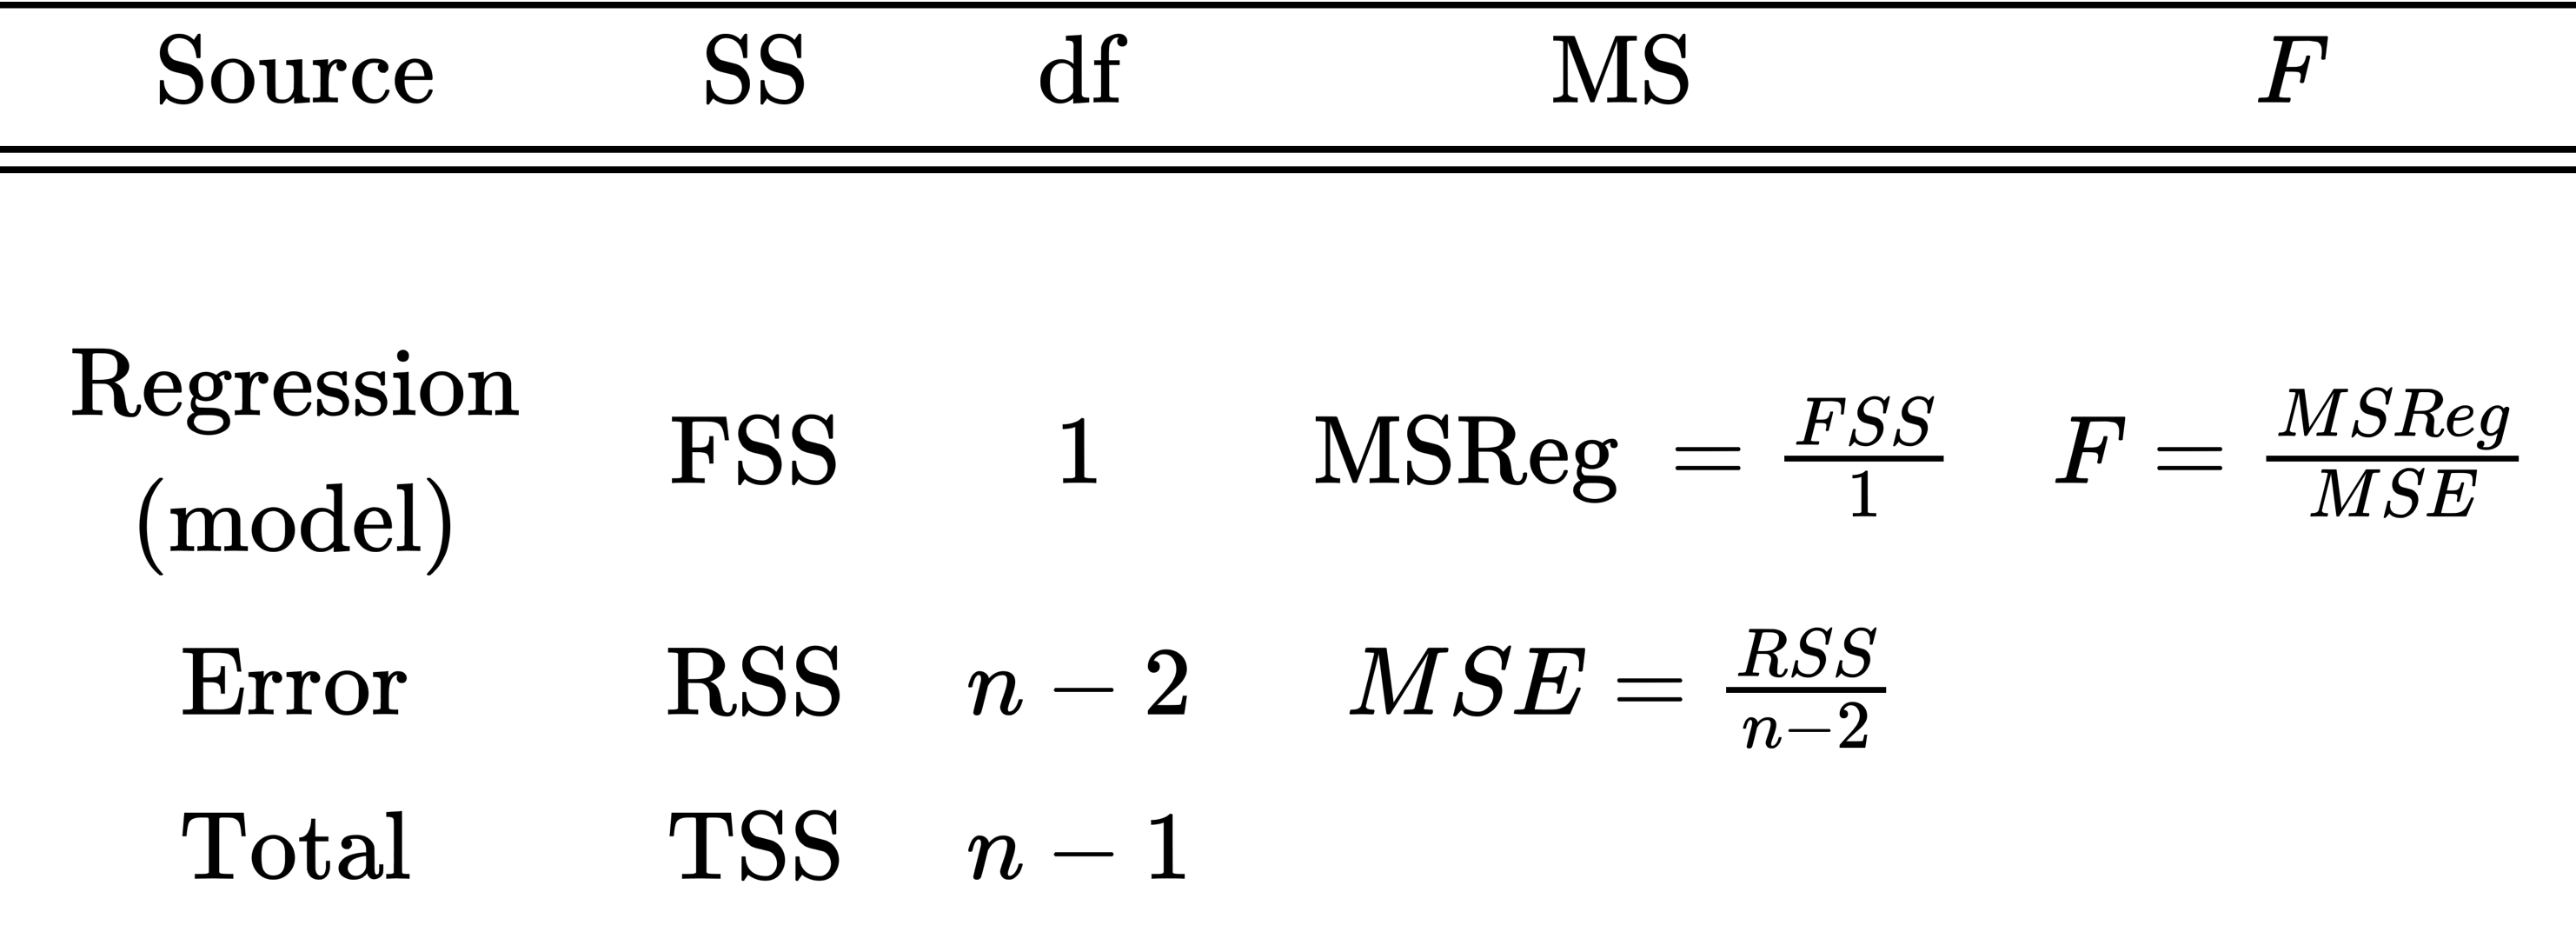
\includegraphics[scale=1]{rendered_image.png}
    \caption{}
    \label{}
\end{figure}\end{center}

\subsubsection{F-Test (equivalent to t-test)}
An alternative way to test for the model parameters is using the $F$ test:
$$
\left\{\begin{array}{l}
H_{0}: \beta_{1}=0 \\
H_{\alpha}: \beta_{1} \neq 0
\end{array}\right.
$$
- Under $H_{0}$, the $F$-test statistic is
$$
F=\frac{\text { MSReg }}{M S E}=\frac{F S S}{R S S /(n-2)} \sim F_{1, n-2}
$$
- It can be shown that the $F$-test statistic is equal to the square of the $t$-test statistic and their $p$-values are the same. So, \textbf{this test is equivalent to the $t$-test before}.

\subsection{Estimation and Prediction}

\subsubsection{Estimation (always reported for a parameter: ${\beta}_0+{\beta}_1x^*=\mathbb{E}(Y|x^*)$)}
1. Estimation: We want to estimate the mean response at $x^*$. This is equivalent to estimate: $\beta_0+\beta_1x^*$\\
2. Accuracy of the estimation: is measured by the expected value of the squared difference between the point estimate and the target.\\
- For estimation the target is $\beta_{0}+\beta_{1} x^{\star}:$
$$
\begin{aligned}
& \mathbb{E}\left(\hat{\beta}_{0}+\hat{\beta}_{1} x^{\star}-\beta_{0}-\beta_{1} x^{\star}\right)^{2} \\
=& \operatorname{Var}\left(\hat{\beta}_{0}+\hat{\beta}_{1} x^{\star}\right) \\
=& \operatorname{Var}\left(\hat{\beta}_{0}\right)+\left(x^{\star}\right)^{2} \operatorname{Var}\left(\hat{\beta}_{1}\right)+2 x^{\star} \operatorname{Cov}\left(\hat{\beta}_{0}, \hat{\beta}_{1}\right) \\
=& \sigma^{2}\left(\frac{1}{n}+\frac{\left(x^{\star}-\bar{x}\right)^{2}}{\sum_{i}\left(x_{i}-\bar{x}\right)^{2}}\right) \\
=& \sigma^{2}\left(\frac{1}{n}+\frac{\left(x^{\star}-\bar{x}\right)^{2}}{S_{x x}}\right)
\end{aligned}
$$

3. Confidence interval: An $(1-\alpha) 100 \%$ Confidence Interval for the Mean Response when $x=x^{\star}$ is given by
$$
\hat{\beta}_{0}+\hat{\beta}_{1} x^{\star} \pm T_{n-2}(\alpha / 2) \hat{\sigma} \sqrt{\frac{1}{n}+\frac{\left(x^{\star}-\bar{x}\right)^{2}}{S_{x x}}}
$$

\subsubsection{Prediction (is reported for the value of a random variable $Y^*$)}
1. Prediction: of an outcome of random variable $Y^*$ at a given value $x^*$ , where $Y^* \sim N( \beta_0 + \beta_1 x^* , \sigma^2 )$\\
2. For prediction the target is $Y^{\star}=\beta_{0}+\beta_{1} x^{\star}+e^{\star}$, where $e^{\star} \sim N\left(0, \sigma^{2}\right)$ This new error $e^{\star}$ is independent of the previous $n$ data points, i.e. is independent of $\left(\hat{\beta}_{0}, \hat{\beta}_{1}\right)$
$$
\begin{aligned}
&\mathbb{E}\left[\left(\hat{\beta}_{0}+\hat{\beta}_{1} x^{\star}-Y^{\star}\right)^{2}\right] \\
&=\mathbb{E}\left[\left(\hat{\beta}_{0}+\hat{\beta}_{1} x^{\star}-\beta_{0}-\beta_{1} x^{\star}-e^{\star}\right)^{2}\right] \\
&=\mathbb{E}\left[\left(\hat{\beta}_{0}+\hat{\beta}_{1} x^{\star}-\beta_{0}-\beta_{1} x^{\star}\right)^{2}\right]+\mathbb{E}\left[\left(e^{\star}\right)^{2}\right] \\
&=\sigma^{2}\left(1+\frac{1}{n}+\frac{\left(x^{\star}-\bar{x}\right)^{2}}{S_{x x}}\right)
\end{aligned}
$$
3. Prediction interval: An $(1-\alpha) 100 \%$ Prediction Interval for $\hat{Y}^{\star}$ when $x=x^{\star}$ is given by
$$
\hat{\beta}_{0}+\hat{\beta}_{1} x^{\star} \pm T_{n-2}(\alpha / 2) \hat{\sigma} \sqrt{1+\frac{1}{n}+\frac{\left(x^{\star}-\bar{x}\right)^{2}}{S_{x x}}}
$$
\subsubsection{Simultaneous Confidence}
$\mu^*=\mathbb{E}[y|x^*]=\beta_0+\beta_1x^*$'s Confidence Interval:
$$I(x^*)=(\hat{\mu}^*\pm T_{n-2}(\frac{\alpha}{2})se(\hat{\mu}^*))$$
Where $$\hat{\mu}^*=\hat{\beta}_0+\hat{\beta}_1x^*\text{ and }se(\hat{\mu}^*)=\hat{\sigma}\sqrt{\frac{1}{n}+\frac{(x^*-\bar{x})^2}{\sum_{i=1}^n(x_i-\bar{x})^2}}$$
If we want confidence intervals at multiple points $(x_1^*, x_2^*, \cdots, x_m^*)$, we can use formula $(1)$ to have confidence intervals at the $m$ points: $I(x_1^*), I(x_2^*), \cdots, I(x_m^*)$.\\
We know that:
$$
\mathbb{P}\left(\mu_{i}^{*} \in I\left(x_{i}^{*}\right)\right)=(1-\alpha)
$$
This is the point-wise coverage probability for $\mu_{i}^{*}$ and formula (1) gives the point-wise CI.\\
What about the simultaneous coverage probability? i.e.:
$$
\mathbb{P}\left(\mu_{i}^{*} \in I\left(x_{i}^{*}\right), \text { for } i=1, \ldots, m\right)=?
$$
To make sure that (for example):
$$
\mathbb{P}\left(\mu_{i}^{*} \in I\left(x_{i}^{*}\right), \text { for } i=1, \ldots, m\right)=.95
$$
we need to set $\alpha=5 \% / m$, which is known as the \textbf{Bonferroni correction}.\\
Let $\mathrm{A}_{k}$ denotes the event that the $k$ th confidence interval covers $\mu_{k}^{*}$ with:
$$
\mathbb{P}\left(\mathrm{A}_{k}\right)=(1-\alpha)
$$
Then we can show:
$$
\begin{aligned}
&\mathbb{P}\left(\text { All Cls cover the corresponding } \mu_{k}^{*} \text { values }\right) \\
&=\mathbb{P}\left(\mathrm{A}_{1} \cap \mathrm{A}_{2} \ldots \cap \mathrm{A}_{m}\right) \\
&=1-\mathbb{P}\left(\mathrm{A}_{1}^{c} \cup \mathrm{A}_{2}^{c} \ldots \cup \mathrm{A}_{m}^{c}\right) \\
&\geq 1-\mathbb{P}\left(\mathrm{A}_{1}^{c}\right)-\ldots-\mathbb{P}\left(\mathrm{A}_{m}^{c}\right) \\
&=1-m \alpha
\end{aligned}
$$
If we choose $\alpha / m$ instead of $\alpha$, the simultaneous coverage probability will be $(1-\alpha)$

\subsubsection{Confidence Band (Larger than CI)}
Ideally we would like to construct a simultaneous confidence band (i.e., $m=\infty$ ) across all $x^{*}$ 's. (Scheffé's Theorem - 2959 ). Let
$$
I(x)=(\hat{r}(x)-c \hat{\sigma}, \hat{r}(x)+c \hat{\sigma})
$$
where
$$
\hat{r}(x)=\hat{\beta}_{0}+\hat{\beta}_{1} x, c \hat{\sigma}=\sqrt{2 F(\alpha, 2, n-2)} \sqrt{\frac{1}{n}+\frac{(x-\bar{x})^{2}}{\sum_{i=1}^{n}\left(x_{i}-\bar{x}\right)^{2}}}
$$
Then,
$$
\mathbb{P}(r(x) \in I(x) \text { for all } x) \geq 1-\alpha
$$
Can we construct a simultaneous prediction band? No!\\
Are confidence bands always wider than point-wise confidence intervals? Yes!
For SLR, at a location $x^{*}$, we have
$$
\begin{aligned}
\text { band } &: \hat{\mu}^{*} \pm \sqrt{2 F(\alpha, 2, n-2)} \operatorname{se}\left(\hat{\mu}^{*}\right) \\
\text { interval } &: \hat{\mu}^{*} \pm T_{n-2}(\alpha / 2) \operatorname{se}\left(\hat{\mu}^{*}\right)
\end{aligned}
$$
$$
\sqrt{2 F(\alpha, 2, n-2)} > T_{n-2}(\alpha / 2)=\sqrt{2 F(\alpha, 1, n-2)}
$$
In fact, for any $\alpha$, we have
$$
T_{m}(\alpha / 2)=\sqrt{2F(\alpha, 1, m)}<\sqrt{k F(\alpha, k, m)}
$$




\subsection{Maximum likelihood estimators with normal error terms}
We start with the statistical model, which is the Gaussian-noise simple linear regression model, defined as follows:\\
1. The distribution of $X$ is arbitrary (and perhaps $X$ is even non-random).\\
2. If $X=x$, then $Y=\beta_{0}+\beta_{1} x+\epsilon$, for some constants ("coefficients", "parameters") $\beta_{0}$ and $\beta_{1}$, and some random noise variable $\epsilon$.\\
3. $\epsilon \sim N\left(0, \sigma^{2}\right)$, and is independent of $X$.\\
4. $\epsilon$ is independent across observations.\\
$$p(y_i|x_i; \beta_0,\beta_1,\sigma^2)=\frac{1}{\sqrt{2\pi\sigma^2}}e^{-\frac{1}{2}(\frac{y_i-(\beta_0+\beta_1x_i)}{\sigma})^2}$$
Given any data set $(x_1, y_1), (x_2, y_2), . . . (x_n, y_n)$, we can now write down the probability density, under the model, of seeing that data:
$$\prod_{i=1}^n p(y_i|x_i; \beta_0,\beta_1,\sigma^2)=\prod_{i=1}^n\frac{1}{\sqrt{2\pi\sigma^2}}e^{-\frac{1}{2}(\frac{y_i-(\beta_0+\beta_1x_i)}{\sigma})^2}=\frac{1}{(2\pi\sigma^2)^{\frac{n}{2}}}e^{-\frac{\sum_{i=1}^n(y_i-(\beta_0+\beta_1x_i))^2}{2\sigma^2}}$$
Take the \textbf{log-likelihood}
$$L(\beta_0,\beta_1,\sigma^2)=-\frac{n}{2}\log{2\pi}-n\log{\sigma}-\frac{1}{2\sigma^2}\sum_{i=1}^n(y_i-(\beta_0+\beta_1x_i))^2$$
Then we can compute the \textbf{Maximum likelihood estimators} $(\hat{\beta}_0,\hat{\beta}_1,\hat{\sigma}^2)$:\\
(1) $(\hat{\beta}_0,\hat{\beta}_1)$,\\
Obviously, maximizing $L(\hat{\beta}_0,\hat{\beta}_1,\hat{\sigma}^2)$ is as same as minimizing $\sum_{i=1}^n(y_i-(\hat{\beta}_0+\hat{\beta}_1x_i))^2$, then the \textbf{Maximum likelihood estimators} is exactly the \textbf{LS estimators}:
$$\begin{aligned}
    &\hat{\beta}_{1}=\frac{\sum_{i=1}^{n}\left(x_{i}-\bar{x}\right)\left(y_{i}-\bar{y}\right)}{\sum_{i=1}^{n}\left(x_{i}-\bar{x}\right)^{2}} \\
    &\hat{\beta}_{0}=\bar{y}-\hat{\beta}_{1} \bar{x}
\end{aligned}$$
(2) $\hat{\sigma}^2$,\\
And the $\hat{\sigma}^2$ is exactly the in-sample mean squared error:
$$\hat{\sigma}^2=\frac{1}{n}\sum_{i=1}^n(y_i-(\hat{\beta}_0+\hat{\beta}_1x_i))^2$$










\section{Multiple Linear Regression}
\subsection{Basic}
$x_{1}, x_{2}, \ldots, x_{p}$ be $p$ predictors of a response $y$.\\
The data will be of the form:
$\begin{array}{ccccc}y_{1} & x_{11} & x_{12} & \cdots & x_{1 p} \\ y_{2} & x_{21} & x_{22} & \cdots & x_{2 p} \\ \vdots & \vdots & \vdots & \ddots & \vdots \\ y_{n} & x_{n 1} & x_{n 2} & \cdots & x_{n p}\end{array}$

Model Equation:
$$
y_{i}=\beta_{1} x_{i 1}+\beta_{2} x_{i 2}+\cdots+\beta_{p} x_{i p}+\varepsilon_{i}, \quad i=1, \ldots, n
$$
where we denote $\mathbf{x}_{\mathbf{i}}=\left(x_{i 1, \ldots, x_{i} p}\right)^{T}$, with $x_{i 1}=1$\\
$\left(\beta_{1}, \beta_{2}, \ldots, \beta_{p} ; \sigma^{2}\right)$ are unknown true parameters.\\
$\beta_{1}$ is the intercept.\\
$\beta_{2}, \beta_{3}, \ldots, \beta_{p}$ are partial slopes.\\
$\sigma^{2}$ is the error variance
\subsubsection{Assumptions of errors}
$\varepsilon_{1}, \varepsilon_{2}, \ldots, \varepsilon_{n}$ are the random errors. They usually assumed to satisfy the same conditions as in simple linear regression:\\
- zero mean: $\mathbb{E}\left(\varepsilon_{i}\right)=0$\\
- uncorrelated: $\left.\operatorname{Cov}\left(\varepsilon_{\mathrm{i}}, \varepsilon_{\mathrm{j}}\right)=0, \mathrm{i} \neq \mathrm{j}\right)$, and\\
- homoscedastic: $\operatorname{Var}\left(\varepsilon_{\mathrm{i}}\right)=\sigma^{2}$ does not depend on $i$ ).

\subsubsection{Matrix Representation}
Matrix Representation of the MLR Model:
$$\begin{array}{cccccc}\mathbf{y}_{n \times 1} & = & \mathbf{X}_{n \times p} & \beta_{p \times 1} & + & \varepsilon_{n \times 1} \\ \uparrow & &\uparrow & \uparrow & &\uparrow \\ \text { Response }& & \text { Design } & \text { Coefficients } & &\text { Error } \\ & & \text { Matrix } & & &\text { Term }\end{array}$$
- $n:$ sample size\\
- $p:$ number of predictors or columns of $X$\\
- By default the intercept is included in the model in which case the first column of $X$ is a vector of 1 's.\\
We set $\mathbb{E}(\varepsilon)=0\text{ and }Cov(\varepsilon)=\sigma^2 \mathbf{I}_n$, then we can infer that
$$\mathbb{E}(y)= \mathbf{X}\beta,\ Cov(y)=\sigma^2 \mathbf{I}_n$$

\subsection{Parameter Estimation $\hat{\beta}=\left(\mathbf{X}^{T} \mathbf{X}\right)^{-1} \mathbf{X}^{T} y$}
- We want to estimate $\beta$, i.e. obtain:
$$
\hat{\beta}=\left(\hat{\beta}_{1}, \hat{\beta}_{2}, \ldots, \hat{\beta}_{p}\right)^{T}
$$
- The LS estimator of $\beta$ minimizes the sum of squared residuals:
$$
R S S=\|y-\mathbf{X} \beta\|^{2}=(y-\mathbf{X} \beta)^{T}(y-\mathbf{X} \beta)
$$
In order to minimize $R S S=(y-\mathbf{X} \beta)^{T}(y-\mathbf{X} \beta)$, we take derivatives with respect to $\beta$ 's and set to zero (as before).\\
$$\frac{\partial R S S}{\partial \beta}=-2 \mathbf{X}_{p \times n}^{T}(y-\mathbf{X} \beta)_{n \times 1}=\mathbf{0}_{p \times 1}$$
$\mathbf{X}^{T}(y-\mathbf{X} \beta)=\mathbf{0} \longrightarrow$ Normal Equations\\
$\left(\mathbf{X}^{T} \mathbf{X}\right) \beta=\mathbf{X}^{T} y$\\
$\hat{\beta}=\left(\mathbf{X}^{T} \mathbf{X}\right)^{-1} \mathbf{X}^{T} y \rightarrow \mathrm{LS}$ Estimators\\
\textbf{Remarks}\\
1. We assume that the rank of $X$ is $p$, i.e. no columns of $X$ is a linear combinations of the other columns of $X$.\\
2. Since $\mathbf{X}$ has rank $p$, the inverse of $\left(\mathbf{X}^{T} \mathbf{X}\right)$ exists.\\
3. if $\left(\mathbf{X}^{T} \mathbf{X}\right)$ is singular the $LS$ solutions is not unique (identifiability problem)

\subsubsection{Fitted Values $\hat{y}_{n \times 1}=\mathbf{H}_{n \times n} y_{n \times 1}$}
$$
\begin{aligned}
\hat{y}_{n \times 1} &=\mathbf{X} \hat{\beta} \\
&=\mathbf{X}\left(\mathbf{X}^{T} \mathbf{X}\right)^{-1} \mathbf{X}^{T} y \\
&=\mathbf{X}\left(\mathbf{X}^{T} \mathbf{X}\right)^{-1} \mathbf{X}^{\top} y\\&=\mathbf{H}_{n \times n} y_{n \times 1}
\end{aligned}
$$
$\mathbf{H}_{n \times n}=\mathbf{X}\left(\mathbf{X}^{T} \mathbf{X}\right)^{-1} \mathbf{X}^{\top}$ is called the hat matrix, since it returns the "y-hat" values.
\subsection{Residuals $\mathbf{r}=(\mathbf{I}-\mathbf{H}) y$, (Sample) error variance $\hat{\sigma}^2=\frac{\mathbf{r}^T \mathbf{r}}{n-p}$}
$$
\mathbf{r}_{n \times 1}=y-\hat{y}=y-\mathbf{H} y=(\mathbf{I}-\mathbf{H}) y
$$
The residuals $\mathbf{r}$ are used to estimate the error variance:
$$
\hat{\sigma}^2=\frac{1}{n-p} \sum_{i} r_{i}^{2}=\frac{\mathbf{r}^T \mathbf{r}}{n-p}=\frac{R S S}{n-p}
$$

\subsection{Properties of residuals}
The LS estimator is the $\beta$ that satisfies the normal equations, that is
$$
\mathbf{X}^{T}(y-\hat{y})=\mathbf{X}^{T}(y-\mathbf{X} \hat{\beta})=\mathbf{0}
$$
This implies the following properties for the residuals, $r_{n \times 1}=y-\mathbf{X} \hat{\beta}$ :
\subsubsection{$\mathbf{X}^{T} \boldsymbol{r}=0$}
1. The cross-products between the residual vector $r$ and each column of $\mathbf{X}$ are zero, i.e.
$$
\begin{aligned}
\mathbf{X}^{T} \boldsymbol{r} &=\mathbf{X}^{T}(\boldsymbol{y}-\mathbf{X} \hat{\boldsymbol{\beta}})=\mathbf{X}^{T} \boldsymbol{y}-\mathbf{X}^{T} \mathbf{X} \hat{\beta} \\
&=\mathbf{X}^{T} \boldsymbol{y}-\left(\mathbf{X}^{T} \mathbf{X}\right)\left(\mathbf{X}^{T} \mathbf{X}\right)^{-1} \mathbf{X}^{T} \boldsymbol{y}=0
\end{aligned}
$$
\subsubsection{$\hat{y}^{T} \boldsymbol{r}=0$}
2. The cross-product between the fitted value $\hat{y}$ and the residual vector $r$ is zero, i.e.
$$
\hat{y}^{T} r=\hat{\beta}^{T} X^{T} r=0
$$
This implies that the residual vector $r$ is \textbf{orthogonal} to each column of $X$ and $\hat{y}$.\\
\subsection{Properties of $\mathbf{H}$}
\subsubsection{$\mathbf{H X}=\mathbf{X}$}
Let $c$ be any linear combination of the columns of $\mathbb{X}$, then
$$
\mathbf{H} c=c
$$
since $\mathbf{H X}=\mathbf{X}\left(\mathbf{X}^{\top} \mathbf{X}\right)^{-1} \mathbf{X}^{T} \mathbf{X}=\mathbf{X}$
\subsubsection{Symmetric: $\mathbf{H}^{T}=\mathbf{H}$}
\textbf{Symmetric}, since $\mathbf{H}^{T}=\left(\mathbf{X}\left(\mathbf{X}^{T} \mathbf{X}\right)^{-1} \mathbf{X}^{T}\right)^{T}=\mathbf{X}\left(\mathbf{X}^{T} \mathbf{X}\right)^{-1} \mathbf{X}^{T}=\mathbf{H}$
\subsubsection{Idempotent: $\mathbf{H H}=\mathbf{H H}^{T}=\mathbf{H}^{\top} \mathbf{H}=\mathbf{H}$}
\textbf{Idempotent}, i.e. $\mathbf{H H}=\mathbf{H H}^{T}=\mathbf{H}^{\top} \mathbf{H}=\mathbf{H} .$ Indeed
$$
\mathbf{H H}=\mathbf{X}\left(\mathbf{X}^{T} \mathbf{X}\right)^{-1} \mathbf{X}^{T} \mathbf{X}\left(\mathbf{X}^{T} \mathbf{X}\right)^{-1} \mathbf{X}^{T}=\mathbf{X}\left(\mathbf{X}^{T} \mathbf{X}\right)^{-1} \mathbf{X}^{T}=\mathbf{H}
$$
\subsubsection{$\mathbf{H}(\mathbf{I}-\mathbf{H})=\mathbf{0}$}
This also implies that $\mathbf{H}(\mathbf{I}-\mathbf{H})=\mathbf{0}_{n \times n}$
\subsubsection{$(\mathbf{I}-\mathbf{H})$ is also symmetric and idempotent}
$$(\mathbf{I}-\mathbf{H})(\mathbf{I}-\mathbf{H})=(\mathbf{I}-\mathbf{H})^T(\mathbf{I}-\mathbf{H})=(\mathbf{I}-\mathbf{H})(\mathbf{I}-\mathbf{H})^T=\mathbf{I}-\mathbf{H}$$
\subsubsection{$\operatorname{trace}(\mathbf{H})=\mathrm{p}$}
$\operatorname{trace}(\mathbf{H})=\mathrm{p}$, the number of $\mathrm{LS}$ coefficients we estimated.

\subsection{Geometric Representation of LS}
\begin{center}\begin{figure}[htbp]
    \centering
    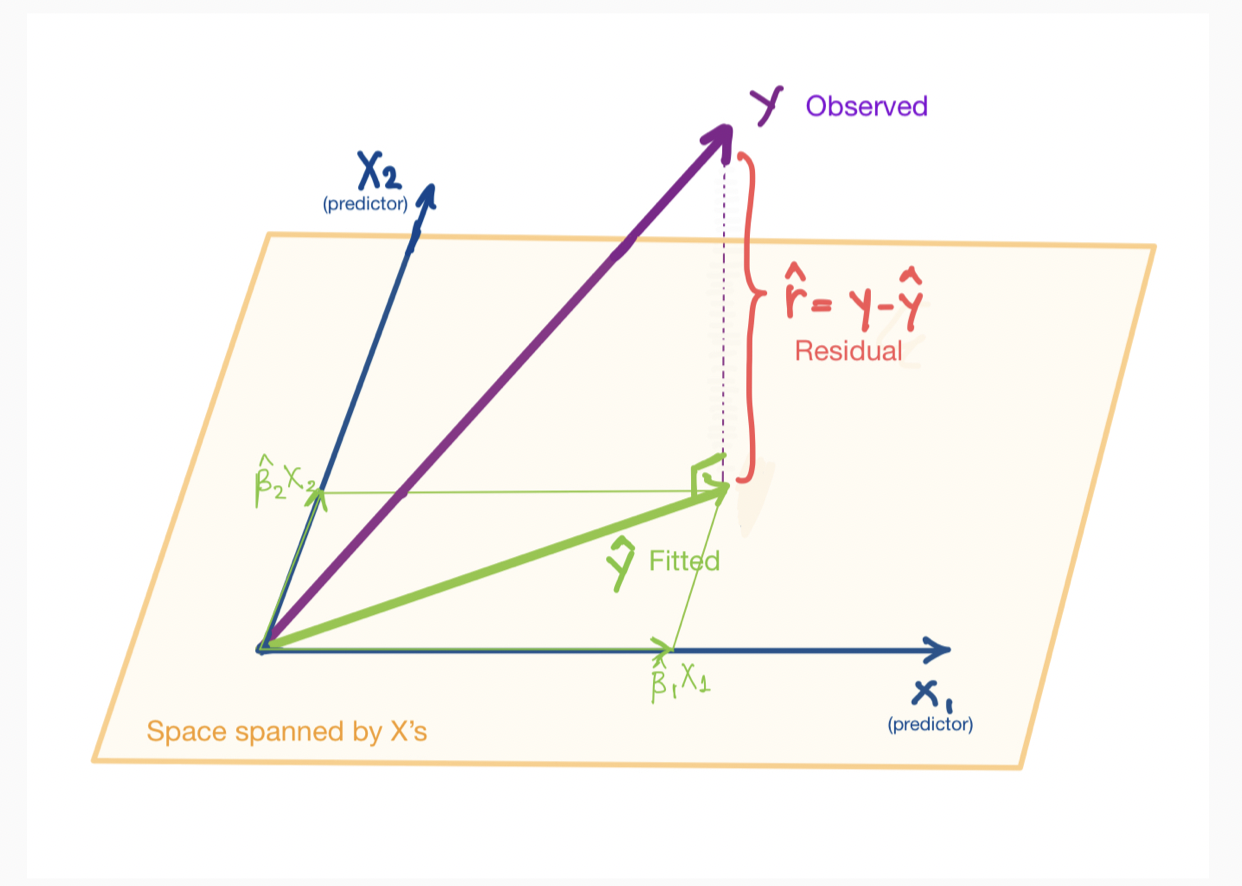
\includegraphics[scale=0.5]{截屏2021-09-05 22.22.04.png}
    \caption{}
    \label{}
\end{figure}\end{center}
\subsubsection{Estimation Space}
- The columns of $\mathbf{X}$ span a $p$-dimensional subspace in $\mathbb{R}^{n}$. This is a subspace that consists of vectors that can be written as linear combinations of the columns of $X$.\\
- The LS squares estimator $\hat{\beta}$ is obtained by minimizing the Euclidean distance between the vectors $\mathbf{y}$ and $\hat{\mathbf{y}}$, i.e. $\|y-\hat{y}\|^{2}$. $\hat{y}$ is the projection of $y$ onto the estimation space.\\
- $\mathbf{H}_{n \times n}$, projection/hat matrix is symmetric, unique, and idempotent.\\
\subsubsection{Error Space}
- The error space is an $(n-p)$-dimensional space that is orthogonal to the estimation space. The projection matrix of the error space is $(\mathbf{I}-\mathbf{H})$.\\
- The residual $\mathbf{r}$ is the projection of $\boldsymbol{y}$ onto the error space, orthogonal to the estimation space. So, $\mathbf{r}$ is orthogonal to any vector in the estimation space, including each column of $X$.\\
- When the intercept is included in the model, then
$$
\sum_{i=1}^{n} r_{i}=0
$$
In general, $\sum_{i=1}^{n} r_{i} X_{i j}=0, j=1, \ldots, p$ due to the normal equations.

\subsection{Coefficient of determination, $R-$Square}
$$
R^{2}=1-\frac{\sum_{i}\left(\hat{y}_{i}-y_{i}\right)^{2}}{\sum_{i}\left(y_{i}-\bar{y}\right)^{2}}=1-\frac{R S S}{T S S}
$$
An equivalent definition is
$$
R^{2}=\frac{\sum_{i}\left(\hat{y}_{i}-\bar{y}\right)^{2}}{\sum_{i}\left(y_{i}-\bar{y}\right)^{2}}
$$
$0 \leq R^{2} \leq 1$
\subsection{Properties of LS Estimators}
\subsubsection{Unbiased: $\mathbb{E}(\hat{\beta})=\beta$}
\begin{equation}
    \begin{aligned}
        \mathbb{E}(\hat{\beta})&=\mathbb{E}(\left(\mathbf{X}^{T} \mathbf{X}\right)^{-1} \mathbf{X}^{T} y)=\left(\mathbf{X}^{T} \mathbf{X}\right)^{-1} \mathbf{X}^{T} \mathbb{E}(y)\\
        &=\left(\mathbf{X}^{T} \mathbf{X}\right)^{-1} \mathbf{X}^{T}\mathbf{X}\beta=\beta
    \end{aligned}
    \nonumber
\end{equation}

\subsubsection{Variance-Covariance Matrix of $\hat{\beta}$: $\operatorname{Cov}(\hat{\beta})=\sigma^{2}\left(\mathbf{X}^{T} \mathbf{X}\right)^{-1}$}
$$\begin{aligned} \operatorname{Cov}(\hat{\beta}) &=\left(\mathbf{X}^{T} \mathbf{X}\right)^{-1} \mathbf{X}^{T} \operatorname{Cov}(\mathbf{y})\left(\left(\mathbf{X}^{\top} \mathbf{X}\right)^{-1} \mathbf{X}^{\top}\right)^{\top} \\ &=\left(\mathbf{X}^{T} \mathbf{X}\right)^{-1} \mathbf{X}^{T} \sigma^{2} \mathbf{X}\left(\mathbf{X}^{\top} \mathbf{X}\right)^{-1} \\ &=\sigma^{2}\left(\mathbf{X}^{T} \mathbf{X}\right)^{-1} \mathbf{X}^{\top} \mathbf{X}\left(\mathbf{X}^{T} \mathbf{X}\right)^{-1} \\ &=\sigma^{2}\left(\mathbf{X}^{T} \mathbf{X}\right)^{-1} \end{aligned}$$
$$se(\hat{\beta}_i)=\hat{\sigma}\sqrt{((\mathbf{X}^T\mathbf{X})^{-1})_{ii}}$$


\subsubsection{$\hat{y}$: $\mathbb{E}(\hat{y})=\mathbf{X}\beta$, $Cov(\hat{y})=\sigma^2 \mathbf{H}$}
\begin{equation}
    \begin{aligned}
        &\mathbb{E}(\hat{y})=\mathbb{E}(\mathbf{X}\left(\mathbf{X}^{T} \mathbf{X}\right)^{-1} \mathbf{X}^{\top}y)=\mathbf{X}\left(\mathbf{X}^{T} \mathbf{X}\right)^{-1} \mathbf{X}^{\top}\mathbf{X}\beta=\mathbf{X}\beta\\
        &Cov(\hat{y})=Cov(\mathbf{H}y)=\mathbf{H}Cov(y)\mathbf{H}^T=\sigma^2\mathbf{H}\mathbf{H}^T=\sigma^2\mathbf{H}
    \end{aligned}
    \nonumber
\end{equation}
\subsubsection{$\mathbf{r}$: $\mathbb{E}(\mathbf{r})=0$, $Cov(\mathbf{r})=\sigma^2 (\mathbf{I}_n-\mathbf{H})$}
\begin{equation}
    \begin{aligned}
        &\mathbb{E}(\mathbf{r})=\mathbb{E}(y-\hat{y})=0\\
        &Cov(\mathbf{r})=Cov(y-\hat{y})=Cov((\mathbf{I}-\mathbf{H})y)=\sigma^2(\mathbf{I}-\mathbf{H})(\mathbf{I}-\mathbf{H})^T=\sigma^2(\mathbf{I}-\mathbf{H})
    \end{aligned}
    \nonumber
\end{equation}
\subsubsection{$\mathbb{E}(\hat{\sigma}^2)=\sigma^2$}
$$\mathbb{E}(\hat{\sigma}^2)=\frac{1}{n-p}\mathbb{E}(\mathbf{r}^T \mathbf{r})=\frac{1}{n-p}\sigma^2(n-p)=\sigma^2$$
$n-p$来自于: 有$p$个元素在H对角中为$1$,其余为$0$,所以$\mathbf{I}_n-\mathbf{H}$对角中有$n-p$个1。所以只有$n-p$个$r_i^2=\sigma^2$
$$\frac{\mathbf{r}^T \mathbf{r}}{\sigma^2}=\frac{RSS}{\sigma^2}\sim \chi^2_{n-p}$$

\subsection{The Gauss-Markov Theorem: LS estimator is the \textbf{BLUE}(best linear unbiased estimator)}
If the errors are 1. Mean zero, 2. umcorrelated, 3. homoscedastic, the LS estimators have \textbf{the lowest variance within the class of linear estimators.}\\
Suppose we are interested in estimating a linear combination of $\beta$ of the form:
$$\theta=\mathbf{c}^T\beta=\sum_{j=1}^pc_j\beta_j$$
LS estimators:
$$\hat{\theta}_{LS}=\mathbf{c}^T\hat{\beta}=\mathbf{c}^T \left(\mathbf{X}^{T} \mathbf{X}\right)^{-1} \mathbf{X}^{T} y$$
This is a \textbf{linear} (linear combination of $y_1,y_2,...,y_n$) and \textbf{unbiased estimator} of $\theta$. Its mean square error can be calculated as:
$$
MSE( \hat{\theta}_{LS} ) = \mathbb{E}( \hat{\theta}_{LS} − \theta)^2 = Var( \hat{\theta}_{LS})$$
\begin{theorem}[Gauss-Markov Theorem]
    $\hat{\theta}_{LS}=\mathbf{c}^T\hat{\beta}$ is the \textbf{BLUE}(best linear unbiased estimator) of the parameter $\mathbf{c}^T\beta$ for any vector $\mathbf{c}\in \mathbb{R}^p$
\end{theorem}

\subsection{Maximum Likelihood Estimation, Distribution of LS estimates}
\subsubsection{$\mathbf{y} \sim \mathbf{N}_{n}\left(\mathbf{X} \beta, \sigma^{2} \mathbf{I}\right)$}
Recall the normality assumption for the regression model:
$$
y_{i}=\mathbf{x}_{i}^{T} \beta+\varepsilon_{i},\quad i=1, \ldots, n, \text { with } \varepsilon_{i} \sim N\left(0, \sigma^{2}\right)
$$
This implies that $\mathbf{y} \sim \mathbf{N}_{n}\left(\mathbf{X} \beta, \sigma^{2} \mathbf{I}\right)$

\subsubsection{LS estimator is the Maximum Likelihood Estimator (MLE)}
We can show that the likelihood function can be written as:
$$
L\left(\beta, \sigma^{2} \mid \mathbf{y}\right) \propto \frac{R S S}{n}^{-\frac{n}{2}}
$$
The value of $\beta$ that maximizes the Likelihood function is \textit{the Maximum Likelihood Estimator (MLE)} of $\beta$. This estimator is equal to the LS estimate of $\beta$.
\subsubsection{$\hat{\beta}\sim \mathbf{N}_{\mathbf{p}}\left(\beta, \sigma^{2}\left(\mathbf{X}^{\top} \mathbf{X}\right)^{-1}\right)$, $\hat{\mathbf{y}}\sim\mathbf{N}_{\mathbf{n}}\left(\mathbf{X} \beta, \sigma^{2} \mathbf{H}\right)$, $\hat{\mathbf{r}}\sim \mathbf{N}_{\mathbf{n}}\left(\mathbf{0}, \sigma^{2}\left(\mathbf{I}_{\mathbf{n}}-\mathbf{H}\right)\right)$}
Recall the assumption for the linear regression model:
$$
\mathbf{y} \sim \mathbf{N}_{\mathbf{n}}\left(\mathbf{X} \beta, \sigma^{2} \mathbf{I}\right)
$$
Any affine transformation of $\mathbf{y}$ will also have a Normal distribution $^{2}$.
We can show that:
$$
\begin{gathered}
\hat{\beta}=\left(\mathbf{X}^{\top} \mathbf{X}\right)^{-1} \mathbf{X}^{\top} \mathbf{y} \sim \mathbf{N}_{\mathbf{p}}\left(\beta, \sigma^{2}\left(\mathbf{X}^{\top} \mathbf{X}\right)^{-1}\right) \\
\hat{\mathbf{y}}=\mathbf{H} \mathbf{y} \sim \mathbf{N}_{\mathbf{n}}\left(\mathbf{X} \beta, \sigma^{2} \mathbf{H}\right) \\
\hat{\mathbf{r}}=\left(\mathbf{I}_{\mathbf{n}}-\mathbf{H}\right) \mathbf{y} \sim \mathbf{N}_{\mathbf{n}}\left(\mathbf{0}, \sigma^{2}\left(\mathbf{I}_{\mathbf{n}}-\mathbf{H}\right)\right)
\end{gathered}
$$
\subsection{$\mathbf{r}$ Residuals’ Properties}
\subsubsection{$\mathbf{r}\in \mathbb{R}^{n-p}$}
Although $\mathbf{r}$ is a vector of dimension $n$, it always lies in a subspace of dimension $(n − p)$.
\subsubsection{$\hat{\sigma}^{2}\sim\sigma^{2} \frac{\chi_{n-p}^{2}}{n-p}$}
r behaves like a random vector with a distribution $\mathbf{N}_{n-p}\left(\mathbf{0}, \sigma^{2} \mathbf{I}_{n-p}\right)$, so we have:
$$
\hat{\sigma}^{2}=\frac{\|\mathbf{r}\|^{2}}{n-p} \sim \sigma^{2} \frac{\chi_{n-p}^{2}}{n-p}
$$
\subsubsection{$\hat{\mathbf{y}}$ and $\boldsymbol{r}$ are independent}
It can be show that $\hat{\mathbf{y}}$ and $\boldsymbol{r}$ are uncorrelated since they are in orthogonal spaces. Since they also have a joint normal distribution, they are independent.

\subsection{Testing Predictors (Coefficients)}
\subsubsection{Testing a Single Predictor $H_0: \beta_j=0$: $t-$test}
Suppose you have a $p$ predictors in your regression model and you want to test the hypothesis:
$$
H_{0}: \beta_{j}=c \text { vs. } H_{\alpha}: \beta_{j} \neq c
$$
- The t-test statistic we use is:
$$
t=\frac{\hat{\beta}_{j}-c}{s e\left(\hat{\beta}_{j}\right)}=\frac{\hat{\beta}_{j}-c}{\hat{\sigma} \sqrt{\left[\left(\mathbf{X}^{\top} \mathbf{X}\right)^{-1}\right]_{j j}}} \sim T_{n-p}
$$
under the null hypothesis $H_{0}$.\\
- p-value $=2 \times$ the area under the curve of a $T_{n-p}$ distribution more extreme than the observed statistic.\\
- The $p$-value returned by the $I m$ function command is for $c=0$.
\subsubsection{Review the degree of freedom}
The degrees of freedom of a $t$-test are determined by the \underline{denominator} of the estimated variance $\hat{\sigma}^{2}$. Consider the following situations:\\
- In STAT 400: Test for $\theta=\alpha$, where $Z_{1}, \ldots, Z_{n} \sim \mathcal{N}\left(\theta, \sigma^{2}\right)$
$$
\frac{\hat{\theta}-\alpha}{\operatorname{se}(\hat{\theta})}=\frac{\overline{\mathbf{Z}}-\alpha}{\sqrt{\hat{\sigma}^{2} / n}} \sim T_{n-1}, \quad \hat{\sigma}^{2}=\frac{\sum_{i}\left(Z_{i}-\bar{Z}\right)^{2}}{n-1}
$$
- In SLR: Test for $\beta_{1}=c$, we have
$$
\frac{\hat{\beta}_{1}-c}{\operatorname{se}\left(\hat{\beta}_{1}\right)}=\frac{\hat{\beta}_{1}-c}{\hat{\sigma} / \sqrt{S_{X X}}} \sim T_{n-2},\quad \hat{\sigma}^{2}=\frac{R S S}{n-2}
$$
- In $M L R$ with $p$ predictors (including the intercept): Test for $\beta_{j}=c$,
$$
\frac{\hat{\beta}_{j}-c}{\operatorname{se}\left(\hat{\beta}_{j}\right)}=\frac{\hat{\beta}_{j}-c}{\hat{\sigma} \sqrt{\left[\left(\mathbf{X}^{T} \mathbf{X}\right)^{-1}\right]_{j j}}} \sim T_{n-p}, \quad\hat{\sigma}^{2}=\frac{R S S}{n-p}
$$

\subsubsection{Testing all predictors: $F-$test}
Testing all predictors
$$
\left\{\begin{array}{l}
H_{0}: \beta_{2}=\beta_{3}=\ldots=\beta_{p}=0 \\
H_{a}: \beta_{j} \neq 0, \quad \text { for some } j, j=2, \ldots, p
\end{array}\right.
$$
- Under the Null hypothesis, the test statistic:
$$
\begin{aligned}
F &=\frac{F S S\left(X_{2}, \ldots, X_{p}\right)}{p-1} \div \frac{R S S\left(X_{2}, \ldots, X_{p}\right)}{n-p} \\
&=\frac{M S(R e g)}{M S(\text { Error })} \sim F_{p-1, n-p}
\end{aligned}
$$
Large values of $F$ lead to conclusion $H_{\alpha}$.\\
- This is the overall $F$ test of whether or not there is a regression relation between the response variable $Y$ and the set of $X$ variables.
\begin{center}\begin{figure}[htbp]
    \centering
    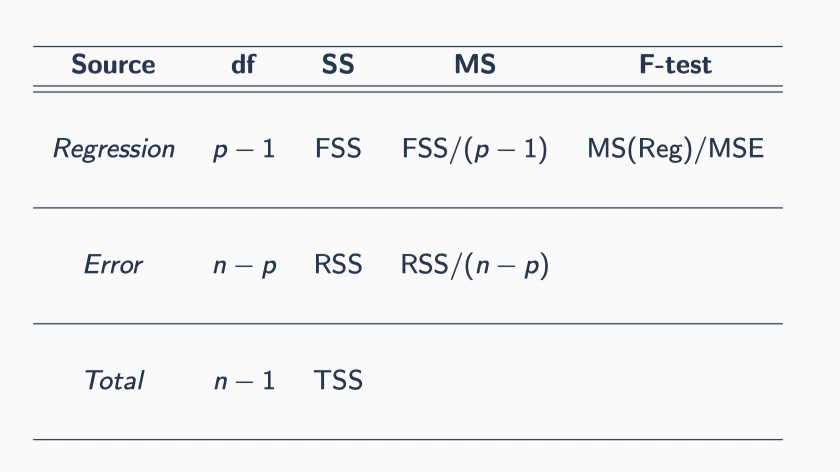
\includegraphics[scale=0.8]{Lec0601.png}
    \caption{}
    \label{}
\end{figure}\end{center}
\subsubsection{Partial $F-$test}
In general, consider the following partition of the design matrix into two sub-matrices $\mathbf{X}_{1}$ and $\mathbf{X}_{2}$, that is
$$
\mathbf{X}_{n \times p}=\left(\mathbf{X}_{1 n \times(p-q)}, \mathbf{X}_{2 n \times q}\right)
$$
The corresponding partition of the regression parameter is:
$$
\beta^{T}=\left(\beta_{1}^{T}, \beta_{2}^{T}\right)
$$
where $\beta_{1}$ is $(p-q) \times 1$ and $\beta_{2}$ is $q \times 1$\\
This partition is used to test the hypothesis:
$$
\left\{\begin{array}{l}
H_{0}: \beta_{2}=\mathbf{0}, \text { i.e., } \quad \mathbf{y}=\mathbf{X}_{1} \beta_{1}+\text { error } \\
H_{\alpha}: \beta_{2} \neq \mathbf{0}, \text { i.e., }\quad \mathbf{y}=\mathbf{X}_{1} \beta_{1}+\mathbf{X}_{2} \beta_{2}+\text { error }
\end{array}\right.
$$
To test this hypothesis, the test statistic is:
$$
F=\frac{\left(R S S_{0}-R S S_{\alpha}\right) / q}{R S S_{\alpha} /(n-p)} \sim F_{q, n-p}
$$
where \textbf{$R R S_{0}=$ Residual sum of squares for the model under $H_{0}$ ; $R R S_{a}=$ Residual sum of squares for the model under $H_{\alpha}$}

\textbf{Numerator}: variation in the data not explained by the reduced model, but explained by the full model.

\textbf{Denominator}: variation in the data not explained by the full model (i.e., not explained by either model), which is used to estimate the error variance.

\textit{Reject $H_{0}$, if $F$ test statistic is large}, that is, the variation missed by the reduced model, when being compared with the error variance, is significantly large.

F-test statistic can be rewirtten:
$$F=\frac{(RSS_{0}-RSS_{\alpha})/q}{RSS_{\alpha}/(n-p)}=\frac{((1-R_R^2)-(1-R_F^2))/(df_F-df_R)}{(1-R_F^2)/df_F}=\frac{(R_F^2-R_R^2)/(df_R-df_F)}{(1-R_F^2)/df_F}$$
Note that this test statistic is not appropriate when the full and reduced regression models do not contain the intercept term $\beta_0$ .

\subsection{Permutation Tests (When the normal distribution hypothesis doesn't hold)}
The distribution of the data is \textit{unknown}.
- A test statistic is a function of the data; denote it $g($ data $)$.\\
- The test statistic tends to take extreme values under the alternative hypothesis $H_{\alpha}$.
\subsubsection{Procedure}
Procedure to conduct a permutation test\\
1. Form the test statistic $g($ data $)$ which tends to take extreme values under the alternative hypothesis.\\
2. Evaluate the test statistic on the observed data, denoted by $g_{0}$.\\
3. Find the distribution of $g($ data $)$, when data are generated from $H_{0}$.\\
4. Calculate the $p$-value, that is the following probability:
\begin{center}
    $\mathbb{P}\left(g(\right.$ data $)$ is more extreme than the observed $g_{0} \mid$ data $\left.\sim H_{0}\right)$
\end{center}

\subsubsection{Calculation of the p-value: Monte Carlo method}
We can obtain an approximation of $\mathbb{E}(Y)$ as follows:\\
1. Generate $N=1000$ samples from this distribution, $Y_{1}, \ldots, Y_{N}$\\
2. Approximate the mean by
$$
\mathbb{E}(Y) \approx \frac{1}{N} \sum_{i=1}^{N} Y_{i}
$$
That is, population mean $\approx$ sample mean (when $N$ is large).\\

This method also works if we want to approximate the expected value of a \textit{function} of a random variable:
$$
\mathbb{E}(f(Y)) \approx \frac{1}{N} \sum_{i=1}^{N} f\left(Y_{i}\right)
$$

\subsection{Confidence Intervals for $\beta_j$, Confidence Region for $\beta$}
\subsubsection{Confidence Intervals for $\beta_j$}
Recall that
$$\hat{\beta}=\left(\mathbf{X}^{\top} \mathbf{X}\right)^{-1} \mathbf{X}^{\top} \mathbf{y} \sim \mathbf{N}_{\mathbf{p}}\left(\beta, \sigma^{2}\left(\mathbf{X}^{\top} \mathbf{X}\right)^{-1}\right)$$
An $(1-\alpha)100\%$ CI(Confidence Interval) for $\beta_j$ can be written as
$$(\hat{\beta}_j \pm T_{n-p}(\frac{\alpha}{2})se(\hat{\beta}_j))=(\hat{\beta}_j \pm T_{n-p}(\frac{\alpha}{2})\hat{\sigma}\sqrt{[\left(\mathbf{X}^{\top} \mathbf{X}\right)^{-1}]_{jj}})$$
\subsubsection{Confidence Region for $\beta$}
$\beta$ is the entire vector,
$$\beta-\hat{\beta}\sim\mathbf{N}_{\mathbf{p}}\left(0, \sigma^{2}\left(\mathbf{X}^{\top} \mathbf{X}\right)^{-1}\right)$$
Thus the quadratic form:
$$\frac{(\beta-\hat{\beta})^T \mathbf{X}^T \mathbf{X}(\beta-\hat{\beta})}{p \hat{\sigma}^2}\sim F_{p,n-p}$$
We can construct a $(1-\alpha)100\%$ confidence region for $\beta$ to be all the points in the following ellipsoid,
$$\frac{(\beta-\hat{\beta})^T \mathbf{X}^T \mathbf{X}(\beta-\hat{\beta})}{p \hat{\sigma}^2}<F(\alpha; p,n-p)$$
Where $F(\alpha; p,n-p)$ is defined to be the point such that $$\mathbb{P}(F_{p,n-p}>F(\alpha; p,n-p))=\alpha$$
\begin{center}\begin{figure}[htbp]
    \centering
    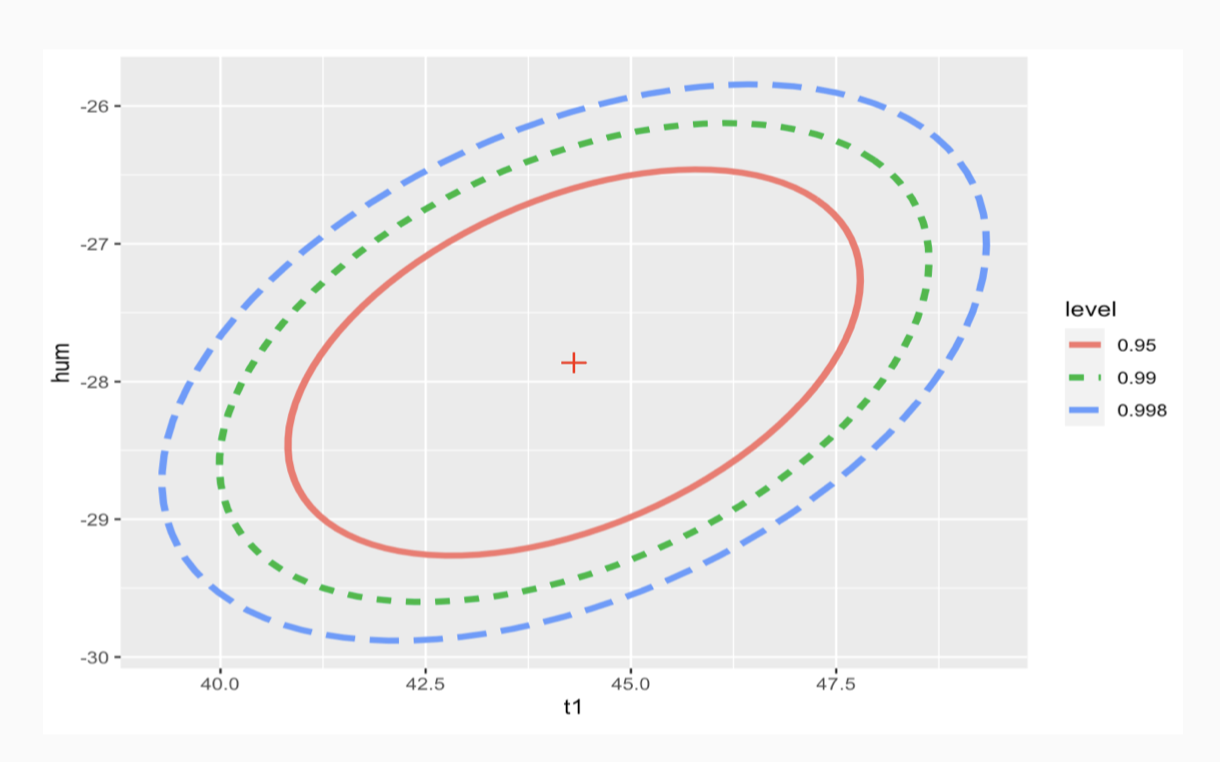
\includegraphics[scale=0.5]{Lec0701.png}
    \caption{}
    \label{}
\end{figure}\end{center}

\subsection{Confidence/Prediction Intervals for New Observations}
Set $\mathbb{E}(Y|x^*)=\mu^*=(x^*)^T\beta$
\subsubsection{Confidence Interval for $\mu^*=(x^*)^T\beta$}
The Gauss-Markov theorem tells us that the BLUE (Best Linear Unbiased Estimate) of $\mu^*$ is:
$$\hat{\mu}^*=(x^*)^T \hat{\beta}=(x^*)^T(X^TX)^{-1}X^Ty$$
Then,
\begin{equation}
    \begin{aligned}
        \mathbb{E}[(\hat{\mu}^*-\mu^*)^2]&=Var(\hat{\mu}^*)\\
        &=\sigma^2(x^*)^T(X^TX)^{-1}x^*\\
        se(\hat{\mu}^*)&=\hat{\sigma}\sqrt{(x^*)^T(X^TX)^{-1}x^*}
    \end{aligned}
    \nonumber
\end{equation}
Where $$\frac{\hat{\mu}^*-\mu}{se(\hat{\mu}^*)} \sim t(n-p)$$
A $(1-\alpha)100\%$ CI (confidence interval) for $\mu^*$ is:
$$\hat{\mu}^*\pm T_{n-p}(\frac{\alpha}{2})se(\hat{\mu}^*)$$
\subsubsection{Prediction Interval for $y^*=(x^*)^T\beta+e^*$}
The best estimate for $y^*$ at a future observation $x^*$ is also
$$\hat{y}^*=(x^*)^T \hat{\beta}$$
Then,
\begin{equation}
    \begin{aligned}
        Var(\hat{y}^*)&=\mathbb{E}[((x^*)^T \hat{\beta}-y^*)^2]\\
        &=\mathbb{E}[((x^*)^T \hat{\beta}-((x^*)^T\beta+e^*))^2]\\
        &=\mathbb{E}[((x^*)^T \hat{\beta}-((x^*)^T\beta)^2]+\mathbb{E}[(e^*)^2]\\
        &=Var(\hat{\mu}^*)+Var(e)\\
        &=\sigma^2[1+(x^*)^T(X^TX)^{-1}x^*]\\
        se(\hat{y}^*)&=\hat{\sigma}\sqrt{1+(x^*)^T(X^TX)^{-1}x^*}
    \end{aligned}
    \nonumber
\end{equation}
Where $$\frac{\hat{y}^*-y^*}{se(\hat{y}^*)} \sim t(n-p)$$
A $(1-\alpha)100\%$ PI (prediction interval) for $y^*$ is:
$$\hat{y}^*\pm T_{n-p}(\frac{\alpha}{2})se(\hat{y}^*)$$

\subsubsection{Mahalanobis distance}
$$\mathbf{X}_{n\times p}=\begin{bmatrix}
    \mathbf{x}_1&\mathbf{x}_2&\cdots&\mathbf{x}_n
\end{bmatrix}^T$$
For any observation vector $\mathbf{x}_{p\times 1}=\begin{pmatrix}
    1\\
    \mathbf{z}
\end{pmatrix}$, where $\mathbf{z}$ denotes the value of predictors without the intercept.\\
We would like to use \textbf{Mahalanobis distance} to quantify the distance between observation vector $\mathbf{x}_{p\times 1}$ and its sample meaning $\bar{\mathbf{x}}$.\\
The sample convariance matrix of $\mathbf{Z}=\begin{bmatrix}
    \mathbf{z}_1&\mathbf{z}_2&\cdots&\mathbf{z}_n\\
\end{bmatrix}$ is:
$$\hat{\Sigma}_{(p-1)\times(p-1)}=\frac{1}{n-1}\sum_{i=1}^n(\mathbf{z}_i-\bar{\mathbf{z}})(\mathbf{z}_i-\bar{\mathbf{z}})^T$$
Then the $(x^*)^T(X^TX)^{-1}x^*$ can be written as
\begin{equation}
    \begin{aligned}
        (x^*)^T(X^TX)^{-1}x^*=\frac{1}{n}+\underline{\frac{1}{n-1}(\mathbf{z}^*-\bar{\mathbf{z}})^T\hat{\Sigma}^{-1}(\mathbf{z}^*-\bar{\mathbf{z}})}
    \end{aligned}
    \nonumber
\end{equation}
The second term in the right hand side ($\frac{1}{n-1}(\mathbf{z}^*-\bar{\mathbf{z}})^T\hat{\Sigma}^{-1}(\mathbf{z}^*-\bar{\mathbf{z}})$) is the so-called Mahalanobis distance from $\mathbf{z}^*$ to the center of the data $\bar{\mathbf{z}}$ (the sample mean).\\
Then we can write,
$$
\begin{aligned}
\operatorname{se}\left(\hat{\mu}^{*}\right) &=\hat{\sigma} \sqrt{\mathbf{x}^{* \top}\left(\mathbf{X}^{\top} \mathbf{X}\right)^{-1} \mathbf{x}^{*}} \\
&=\hat{\sigma} \sqrt{\frac{1}{n}+\frac{1}{n-1}\left(\mathbf{z}^{*}-\overline{\mathbf{z}}\right)^{T} \hat{\Sigma}^{-1}\left(\mathbf{z}^{*}-\overline{\mathbf{z}}\right)} \\
se\left(\hat{y}^{*}\right) &=\hat{\sigma} \sqrt{1+\left(\mathbf{x}^{*}\right)^{\top}\left(\mathbf{X}^{\top} \mathbf{X}\right)^{-1} \mathbf{x}^{*}} \\
&=\hat{\sigma} \sqrt{1+\frac{1}{n}+\frac{1}{n-1}\left(\mathbf{z}^{*}-\overline{\mathbf{z}}\right)^{T} \hat{\Sigma}^{-1}\left(\mathbf{z}^{*}-\overline{\mathbf{z}}\right)}
\end{aligned}
$$
Since $\operatorname{se}\left(\hat{y}^{*}\right)$ has an extra 1, when the sample size $n$ goes to infinity,
$$
\begin{aligned}
&\operatorname{se}\left(\hat{\mu}^{*}\right) \rightarrow 0 \\
&\operatorname{se}\left(\hat{y}^{*}\right) \rightarrow \sigma
\end{aligned}
$$

\section{MLR: unusual observations}
Recall, that we can write the MLR model as:
$$
\mathbf{y} \sim \mathcal{N}\left(\mathbf{X} \beta, \sigma^{2} \mathbf{I}_{n}\right)
$$
$-$ Error: assumed to be iid, $\varepsilon_{i} \sim \mathcal{N}\left(0, \sigma^{2}\right)$\\
$-$ Model: assumed to be linear in the parameters, i.e., $\mathbb{E}(\mathbf{y})=\mathbf{X} \beta$\\
We might have unusual observations.




\subsection{High leverage points: $h_i\geq \frac{2p}{n}$}
\subsubsection{Leverage Points}
The diagonal elements of $\mathbf{H}=\mathbf{X}\left(\mathbf{X}^{T} \mathbf{X}\right)^{-1} \mathbf{X}^{\top}$,
$$
h_{i}=H_{i i}=\mathbf{x}_i\left(\mathbf{X}^{T} \mathbf{X}\right)^{-1} \mathbf{x}_i^{\top}=\frac{Var(x_i^T \hat{\beta})}{\sigma^2}
$$
are called \textbf{leverages} and are very useful diagnostics.
$h_{i}$ gives a measure (invariant under any affine transformation of $\mathbf{X}$ ) of how far the $i$-th observation is from the center of the data (in the $X$-space).\\
For simple linear regression:
$$
h_{i}=\frac{1}{n}+\frac{\left(x_{i}-\bar{x}\right)^{2}}{\sum_{i}\left(x_{i}-\bar{x}\right)^{2}}
$$
In general:
$$
\begin{aligned}
h_{i} &=\mathbf{x}_{\mathbf{i}}^{\boldsymbol{T}}\left(\mathbf{X}^{\top} \mathbf{X}\right)^{-1} \mathbf{x}_{\mathbf{i}} \\
&=\frac{1}{n}+\frac{1}{n-1}\left(\mathbf{z}_{i}-\overline{\mathbf{z}}\right)^{T} \hat{\boldsymbol{\Sigma}}^{-1}\left(\mathbf{z}_{i}-\overline{\mathbf{z}}\right)
\end{aligned}
$$
where
$$
\hat{\Sigma}_{(p-1) \times(p-1)}^{-1}=\frac{1}{n-1} \sum_{i=1}^{n}(\mathbf{z}-\overline{\mathbf{z}})(\mathbf{z}-\overline{\mathbf{z}})^{T}
$$
is the sample covariance of the $(p-1)$ predictor variables. The second term in the right hand side ($\frac{1}{n-1}\left(\mathbf{z}_{i}-\overline{\mathbf{z}}\right)^{T} \hat{\boldsymbol{\Sigma}}^{-1}\left(\mathbf{z}_{i}-\overline{\mathbf{z}}\right)$) is the so-called \textbf{Mahalanobis distance} from $\mathbf{z}_{i}$ to the data center $\overline{\mathbf{z}}$
\subsubsection{Properties of the Leverage: $0<h_{i}<1, \quad \sum_{i} h_{i}=p$}
Recall that the hat matrix is idempotent $\mathbf{H}=\mathbf{H H}^{\top}$ and has $\operatorname{tr}(\mathbf{H})=p$\\
These imply that
$$
\sum_{i} h_{i}=p \text { and } \sum_{j} H_{i j}^{2}=h_{i}
$$
For a given $i$ we can decompose the last sum as follows:
$$
\begin{gathered}
\sum_{j} H_{i j}^{2}=H_{i i}^{2}+\sum_{i \neq j} H_{i j}^{2}=h_{i} \\
\Rightarrow \sum_{i \neq j} H_{i j}^{2}=h_{i}\left(1-h_{i}\right) \Rightarrow h_{i}\left(1-h_{i}\right)>0
\end{gathered}
$$
From this we can conclude the following properties of $h_{i}$ :
$$
0<h_{i}<1, \quad \sum_{i} h_{i}=p
$$

\subsubsection{Fitted Values and Leverage: $Var(\hat{y}_i)=\sigma^2 h_i,\ Var(r_i)=\sigma^2(1-h_i)$}
Recall the equation $\hat{\mathbf{y}}=\mathbf{H}\mathbf{y}$.\\
\begin{equation}
    \begin{aligned}
        \hat{y}_i&=\sum_{t=1}^nH_{it}y_t\\
        &=h_iy_i+\sum_{t\neq i}^nH_{it}y_t
    \end{aligned}
    \nonumber
\end{equation}
This means that $h_i=\frac{d \hat{y}_i}{d y_i}$\\
When $h_i$ is \textbf{large (close to 1)}, $\hat{y}_i$ relies heavily on $y_i$ (instead of using the information from other data points), therefore $\hat{y}_i$ will be “forced” to be \textbf{close} to the observed $y_i$.\\
Consequently, the variance for the residual $r_i$ will be small, and the variance for the fit $\hat{y}_i$ will be large (since the fit from another data set would be quite different).
$$Var(\hat{y}_i)=\sigma^2 h_i,\ Var(r_i)=\sigma^2(1-h_i)$$

\subsubsection{High-leverage Points: $h_i\geq \frac{2p}{n}$}
\textit{Good high-leverage points}: its $y$ point follows the pattern of the rest of the data, but with an $x_i$ value that is far away from the sample mean.\\
\textit{Bad high-leverage points}: its $y$ value does not follow the pattern suggested by the rest of the data; the LS fitting might change a lot if we remove this point.\\

\subsection{Residuals: Standardized Residuals vs. Studentized residuals}
The residuals $r_i=y_i-\hat{y}_i$ do not have a constant variance. So they need to be standardized.
\subsubsection{Difference between $\varepsilon$ and $\mathbf{r}$}
$\varepsilon$ : true residuals (our theoretical quantities)\\
$\mathbf{r}$ : estimated residuals
- Both residuals are normally distributed, but:
$$
\varepsilon \sim \mathcal{N}_{n}\left(\mathbf{0}, \sigma^{2} \mathbf{I}_{n}\right), \quad \mathbf{r} \sim \mathcal{N}_{n}\left(\mathbf{0}, \sigma^{2}\left(\mathbf{I}_{n}-\mathbf{H}\right)\right)
$$
where $\mathbf{H}$ is the projection/hat matrix.\\
- The errors $\varepsilon_{i}$ 's have equal variance and are independent, while the residuals $r_{i}$ 's have unequal variance and are correlated.\\
$-\mathbb{E}(\varepsilon)=\mathbb{E}(\mathbf{r})=\mathbf{0} .$ But
$$
\sum_{i} \varepsilon_{i} \neq 0, \quad \sum_{i} r_{i}=0
$$
(by default we assume an intercept is included in the model)
\subsubsection{Standardized Residuals: $
r_{i}^{*}=\frac{r_{i}}{\hat{\sigma} \sqrt{1-h_{i}}}$}
Since $r_{i} \sim \mathcal{N}\left(0, \sigma^{2}\left(1-h_{i}\right)\right)$, it is reasonable to consider a standardization of the residuals in this form:
$$
r_{i}^{*}=\frac{r_{i}}{\hat{\sigma} \sqrt{1-h_{i}}}, \quad i=1, \ldots, n
$$
- $\sum_{i} r_{i}^{*}$ is no longer zero.\\
- Since the $r_{i}$ is not independent of $\hat{\sigma}$, each $r_{i}^{*}$ is \textbf{not distributed as a $T$ distribution}.\\
- As an approximation, we can view the $r_{i}^{*}$ 's as iid $\mathcal{N}(0,1)$ random variables, although they are not Normally distributed and they are slightly correlated.

\subsubsection{Studentized Residuals: $
t_{i}=r_{i}^{*}\left(\frac{n-p-1}{n-p-r_{i}^{* 2}}\right)^{1 / 2}
$}
- The studentized residuals are based on the idea of leave-one-out (also know as jackknife residuals).\\
- Here is the leave-one-out idea:\\
1. Run a regression model on the $(n-1)$ samples with the $i$-th sample $\left(x_{i}, y_{i}\right)$ removed.\\
2. Denote the leave-one-out estimates of the regression coefficient and error variance by $\hat{\beta}_{(i)}$ and $\hat{\sigma}_{(i)}$, where the notation (i) means "excluding the $i$-th observation."\\
3. Then, check the discrepancy between observations $y_{i}$ and the fitted value $\hat{y}_{(i)}=\mathbf{x}^{T} \hat{\beta}_{(i)}$\\
- Define the Studentized Residuals as:
$$
t_{i}=\frac{y_{i}-\hat{y}(i)}{\hat{\sigma}_{(i)}\left(1+x_{i}^{T}\left(\mathbf{X}_{(\mathbf{i})}^{\top} \mathbf{X}_{(i)}\right)^{-1} x_{i}\right)^{1 / 2}}=\frac{y_{i}-\hat{y}_{(i)}}{\hat{\sigma}_{(i)} \sqrt{1-h_{i}}}
$$
which follows a $T_{n-p-1}$ distribution if $y_{i} \sim \mathcal{N}\left(\mathbf{x}_{i}^{T} \beta, \sigma^{2}\right)$\\
- One can also show that $r_{i}^{*}$ and $t_{i}$ are a monotone transformation of each other.\\
- We do not need to run the model $n$ times to get the estimates $\hat{\beta}_{(i)}$ and $\hat{\sigma}_{(i)}$ since it can be shown that:
$$
t_{i}=r_{i}^{*}\left(\frac{n-p-1}{n-p-r_{i}^{* 2}}\right)^{1 / 2}
$$

\subsection{Outlier (Large $|r_i^*|$)}
\subsubsection{Outlier test}
Outliers are observations that do not fit the model, but Outliers are not necessarily observations with large residuals.\\
We need to used the studentized residuals for the outlier test.\\
Under the Null hypothesis $H_0$,
$$t_i\sim T_{n-p-1}$$
We can use t-test to test the $i^{th}$ observation: form a PI at $x_i$.\\
(an example of data snooping)\\
Large $|r_i^*|$ $\Rightarrow$ Large $|t_i|$ $\Rightarrow$ Reject Null hypothesis $\Rightarrow$ Outlier
\subsubsection{Bonferroni Correction}
Suppose we are testing $m$ hypothesis sinultaneously.\\
For each test, we use a significant level $\alpha$. That is, the chance to make a \textbf{overall} Type I error is $\alpha$.\\
Suppose we want to control the overall type I error rate (for all $m$ tests) to be $95\%$.\\
We should set the individual significance levels to be $\alpha = 5\%/m$
\subsubsection{What we should do with outliers?}
Points should not be routinely deleted simply because they do not fit the model. No data snooping!\\
Outliers, as well as other unusual observations discussed here, often flag potential problems of the current model. \textbf{Instead of dropping them, maybe, try a new alternative model.}

\subsection{Highly Influential Points: Large $D_i=\frac{{r_i^*}^2}{p}(\frac{h_i}{1-h_i})$ \quad ($D_i\geq 1$)}
\subsubsection{Influential observations}
Observations whose removal greatly affects the regression analysis are called \textbf{influential observations}.\\
An \textbf{influential observations} may be (or may not) an \textbf{outlier} or a \textbf{high-leverage observation}; or may be both: an outlier and a high-leverage observation.\\
We will use the \textbf{Cook's distance} to detect influential observations.
$$
D_{i}=\frac{\left\|\mathbf{X} \hat{\beta}-\mathbf{X} \hat{\beta}_{(i)}\right\|^{2}}{p \hat{\sigma}^{2}}=\frac{\left\|\hat{\mathbf{y}}-\hat{\mathbf{y}}_{(i)}\right\|^{2}}{p \hat{\sigma}^{2}}=\frac{r_{i}^{* 2}}{p}\left(\frac{h_{i}}{1-h_{i}}\right)
$$
which indicates that highly influential points are either outliers (large $\left.\left|r_{i}^{*}\right|\right)$ or high-leverage points (large $h_{i}$) or both.\\
A rule-of-thumb: observations with $D_{i} \geq 1$ are highly influential.

\section{Diagnostics: Checking Assumptions}
\subsection{Assimption}
$$\mathbf{Y}=\beta \mathbf{X}+\varepsilon,\ \text{where }\varepsilon\sim^{IID} \mathcal{N}(0,\sigma^2)$$
1. Constant Variance (Homoscedasticity)\\
2. Normality\\
3. Uncorrelated errors (No-Autocorrelation)\\
4. Linearity: $\mathbb{E}(y)=\mathbf{X}\beta$

\subsection{Check Constancy of Variance(Homoscedasticity)}
\subsubsection{Method 1: graph \textit{residuals} against \textit{Fitted Values} $\hat{y}$}
\textbf{SLR}:
\begin{center}\begin{figure}[htbp]
    \centering
    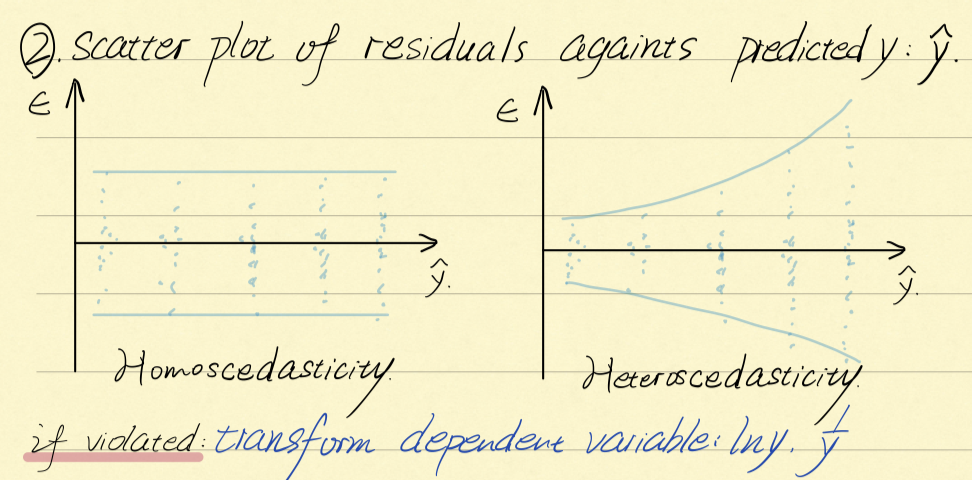
\includegraphics[scale=0.7]{check1.png}
    \caption{}
    \label{}
\end{figure}\end{center}
\textbf{MLR}:\\
If the variance is constant, the residuals will look like a football-shaped cloud. Check residual plots and look for a “fan” type shape or trends.\\
\begin{center}\begin{figure}[htbp]
    \centering
    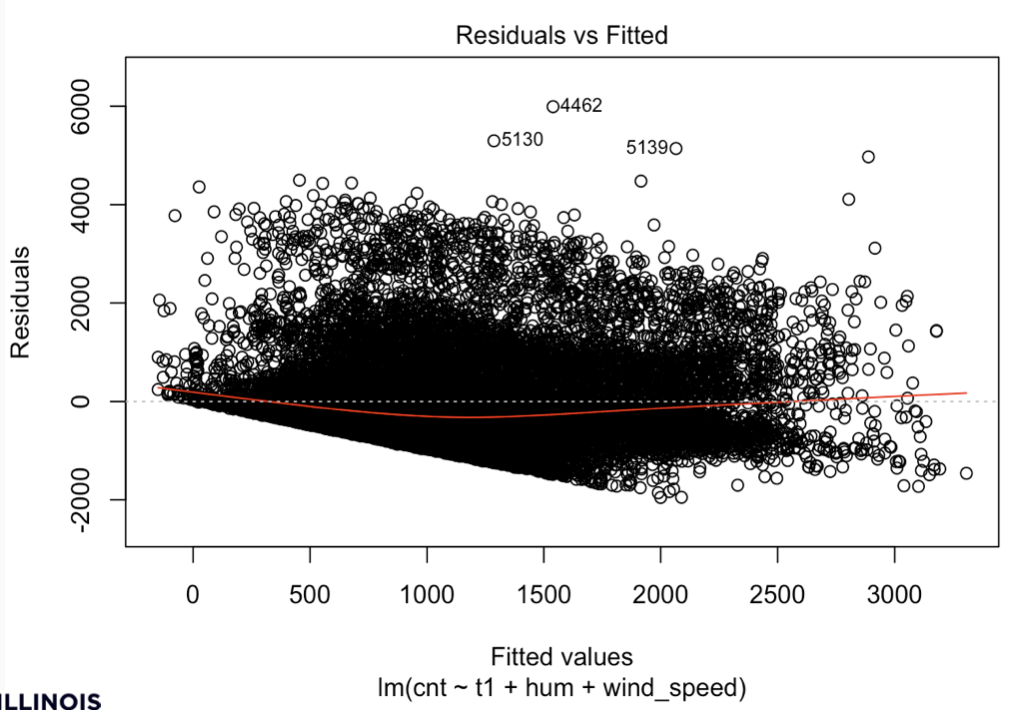
\includegraphics[scale=0.5]{check5}
    \caption{}
    \label{}
\end{figure}\end{center}


\subsubsection{Method 2: Breusch-Pagan Test}
$$\text{BP}=nR^2$$
$$
    H_0:\text{BP}\sim \chi^2_{p-1} \text{ (asymptotically)}
$$

\subsubsection{Remedial measure: Variance Stabilizing Transformations $\sqrt{Y}$, $\log{Y}$, $\frac{1}{Y}\text{ or }\frac{1}{Y+1}$}
\textbf{SLR}:\\
If violates Homoscedasticity: Transform \textit{dependent variable}: $\ln{y}, \frac{1}{y}$\\

\textbf{MLR}:\\
Find a transformation of the response, $h(Y )$, to achieve constant variance.\\
How does it work?\\
- Suppose $h$ is a smooth function.\\
- Using Taylor's theorem, the expansion of $h(Y)$ around $\mathrm{E}(Y)$ is:
$$
h(Y)=h(\mathbf{E}(Y))+h^{\prime}(\mathbf{E}(Y))(Y-\mathbf{E}(Y))+\text { Remainder }
$$
- The \underline{remainder} is assumed small with high probability and we can ignore it:
$$
\operatorname{Var}(\mathrm{h}(\mathrm{Y})) \approx\left(\mathrm{h}^{\prime}(\mathrm{E}(\mathrm{Y}))\right)^{2} \operatorname{Var}(\mathrm{Y})
$$
- We want to choose a transformation $h$ such that $\operatorname{Var}(\mathrm{h}(Y))$ is approximately constant.\\

\textbf{Example 1}:\\
- Suppose that the variance of $Y$ is proportional to the mean of $Y$, i.e., $\operatorname{Var}(Y) \propto E(Y)$\\
- Select $h$ such that:
$$
h^{\prime}(z)=\frac{1}{\sqrt{z}} \Rightarrow h(z) \propto \sqrt{z}
$$
- When plugging-in the value of $h^{\prime}(z)$ evaluated at $E(Y)$ in the variance of $h(Y)$ equation, the variance of $h(Y)$ will be approximately constant. Indeed,
$$
\operatorname{Var}(\sqrt{Y}) \approx\left(\frac{1}{\sqrt{E(Y)}}\right)^{2} \operatorname{Var}(Y)=\frac{\operatorname{Var}(Y)}{E(Y)} \approx \text { const }
$$\\

\textbf{Example 2}:\\
- Suppose that the variance of $Y$ is proportional to the squared mean of $Y$, i.e., $\operatorname{Var}(Y) \propto(E(Y))^{2}$.\\
- Select $h$ such that:
$$
h^{\prime}(z)=\frac{1}{z} \Rightarrow h(z)=\log (z)
$$
- Then,
$$
\operatorname{Var}(\log Y) \approx \frac{1}{(\mathrm{E}(\mathrm{Y}))^{2}} \operatorname{Var}(\mathrm{Y}) \approx \text { const }
$$\\

\textbf{Example 3:}\\
$\operatorname{Var}(Y) \propto(E(Y))^{4}$.\\
$$h(Y)=\frac{1}{Y}\text{ or }\frac{1}{Y+1}$$






\subsection{Check Normality}
\subsubsection{Method 1: Histogram, graph $residuals$ against its frequency}
\begin{center}\begin{figure}[htbp]
    \centering
    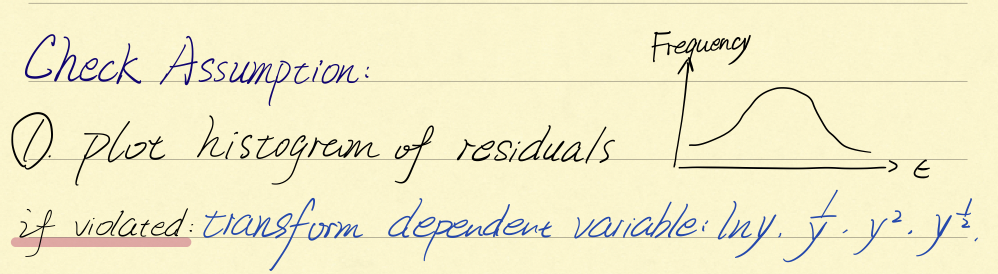
\includegraphics[scale=0.7]{check2.png}
    \caption{}
    \label{}
\end{figure}\end{center}
If violates Normality: Transform \textit{dependent variable}: $\ln{y}, \frac{1}{y},y^2,\sqrt{y}$




\subsubsection{Method 2: QQ-Plot, graph $residuals$ against its frequency}
- Suppose that we have a sample $z_{1}, z_{2}, \ldots, z_{n}$.\\
- We wish to examine the hypothesis that the z's are a sample from a normal distribution with mean $\mu$ and variance $\sigma^{2}$.\\
\textbf{QQ-Plot}:\\
1. Order the z's: $z_{(1)}, z_{(2)}, \ldots, z_{(n)}$.\\
2. Compute $u_{i}=\Phi^{-1}\left(\frac{i}{n+1}\right)$, where $\Phi$ is the cdf of the $N(0,1)$ and $i$ is the order if the data $(i=1,2, \ldots, n)$.\\
3. Plot $z_{(i)}$ against $u_{i}$.\\
$\Rightarrow$ If the z's are normal, the plot should be approximately a straight line.
\begin{center}\begin{figure}[htbp]
    \centering
    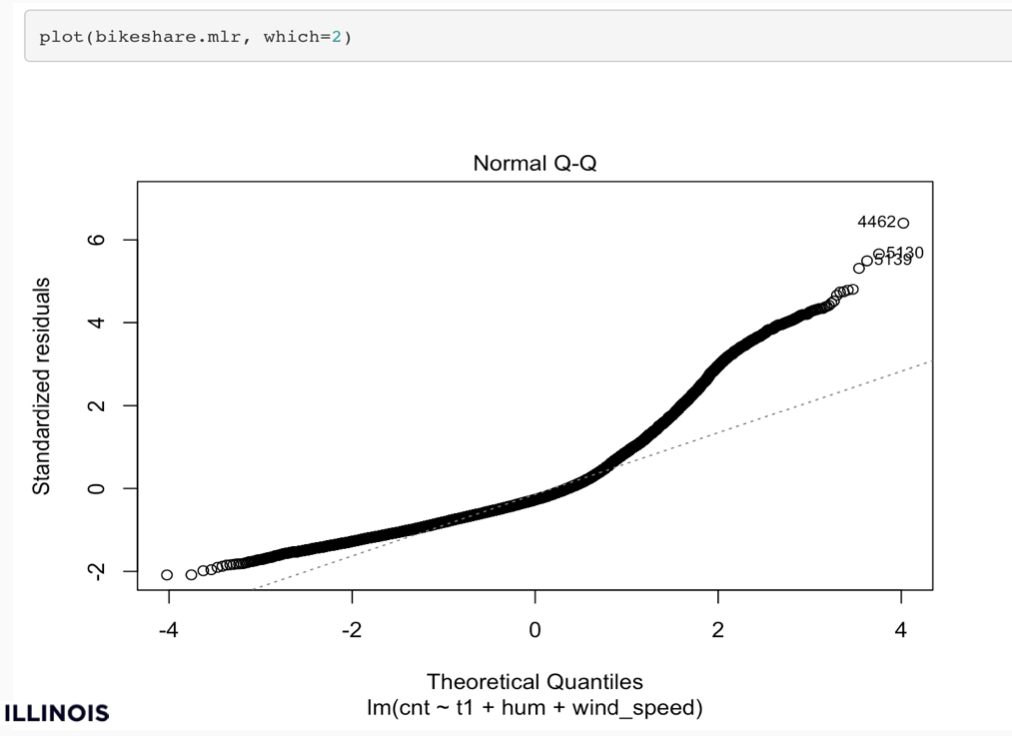
\includegraphics[scale=0.7]{check7.png}
    \caption{}
    \label{}
\end{figure}\end{center}

\subsubsection{Method 3: Shapiro-Wilk Test (good for $n \leq 50$)}
$$W=\frac{(\sum_{i=1}^n a_i r_{(i)})^2}{\sum_{i=1}^n(r_i-\bar{r})^2}$$
where $r_{(i)}$ is the $i$th largest value of the $r_i$’s and the $a_i$ terms are calculated using the means, variances, and covariances of the $r_i$s.\\
\textbf{Small values of $W$} will lead to rejection of the null hypothesis.

\subsubsection{Method 4: Kolmogorov-Smirnov Test (good for $n > 50$)}
$$D_n=\sup_x |F_n(x)-\Phi(x)|$$
where $\Phi(x)$ is the cdf of the Normal and $F_n$ the empirical distribution function $F_n$ for $n$ i.i.d. ordered observations $X_i$ is defined as
$$F_n(x)=\frac{1}{n}\sum_{i=1}^n \mathbf{1}_{[-\infty,x]}(X_i)$$
\textbf{Small values of $D$} will lead to rejection of the null hypothesis.

\subsubsection{Remedial measure: Box-Cox Transformations of $Y$}

Suppose each $y_i>0$, and consider the following transformation:
$$g_\lambda(y)=\left\{\begin{matrix}
    \frac{y^\lambda-1}{\lambda},&\lambda\neq0\\
    \log(y),& \lambda=0
\end{matrix}\right.$$
Choose $\lambda$ that maximizes the likelihood of the data, under the assumption that the transformed data $g_{\lambda}(\mathbf{y})$ has a normal distribution:
$$
g_{\lambda}(\mathbf{y})=\mathbf{X} \beta+\varepsilon, \quad \varepsilon \sim N_{n}\left(\mathbf{0}, \sigma^{2} \mathbf{l}\right)
$$
- The log-likelihood function for $\lambda \neq 0$ is:
$$
\ell(\lambda)=-\frac{n}{2} \log \left(R S S_{\lambda} / n\right)+(\lambda-1) \sum_{i=1}^{n} \log \left(y_{i}\right)
$$
where $R S S_{\lambda}$ is the $R S S$ when $g_{\lambda}(\mathbf{y})$ is the response, and for $\lambda=0$ is:
$$
\ell(0)=-\frac{n}{2} \log \left(R S S_{0} / n\right)-\sum_{i=1}^{n} \log \left(y_{i}\right)
$$
The second term in these log-likelihood function corresponds to the Jacobian of the transformation.\\

In \textbf{R}, we can graph the log-likelihood as a function of $\lambda (L(\lambda))$ versus $\lambda\in (−2, 2)$ and then pick the maximizer $\hat{\lambda}$.\\
\begin{center}\begin{figure}[htbp]
    \centering
    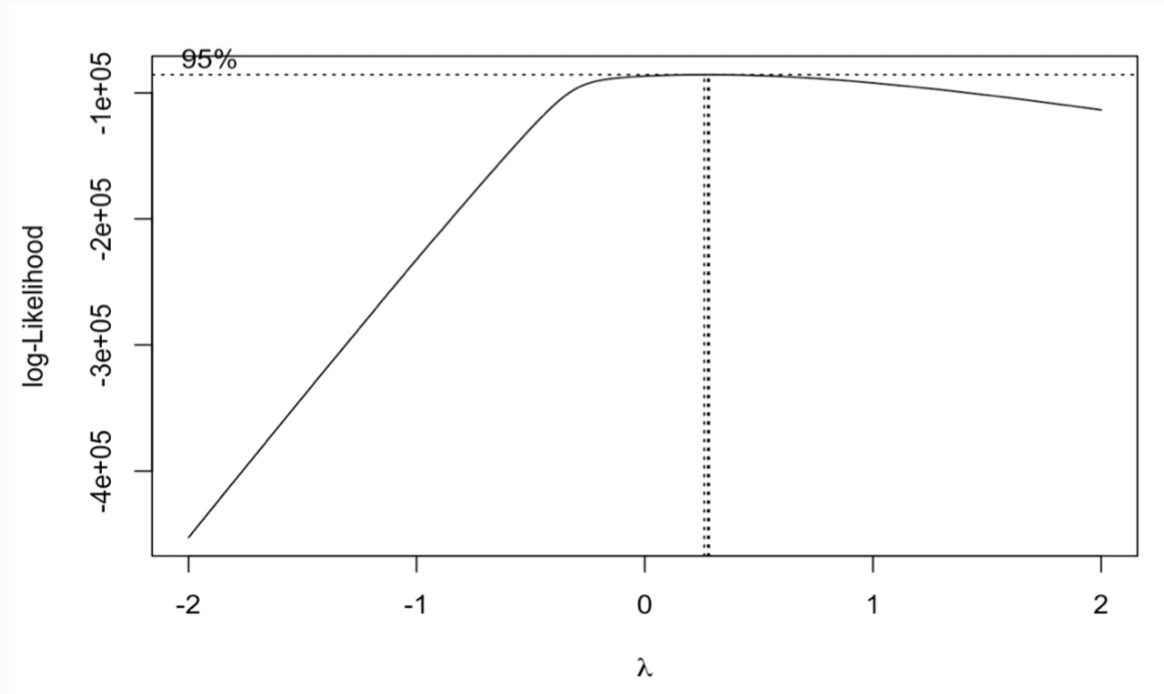
\includegraphics[scale=0.5]{check8.png}
    \caption{}
    \label{}
\end{figure}\end{center}
It is common to round $\hat{\lambda}$ to a nearby value like:
$$−1, −0.5, 0, 0.5, \text{ or } 1 $$then the transformation defined by $\hat{\lambda}$ is easier to interpret.

To answer the question whether we really need the transformation $g_\lambda$, we can do hypothesis testing $(H_0 : \lambda = 1)$, or equivalently construct a Confidence Interval for $\lambda$ as follows:
$$\{\lambda: L(\lambda)>L(\hat{\lambda})-\frac{1}{2}\chi_1^2(1-\alpha)  \}$$

















\subsection{Checking Serial Dependence}
\subsubsection{Method 1: graph $residuals$ against index variable(time or case number)}
\begin{center}\begin{figure}[htbp]
    \centering
    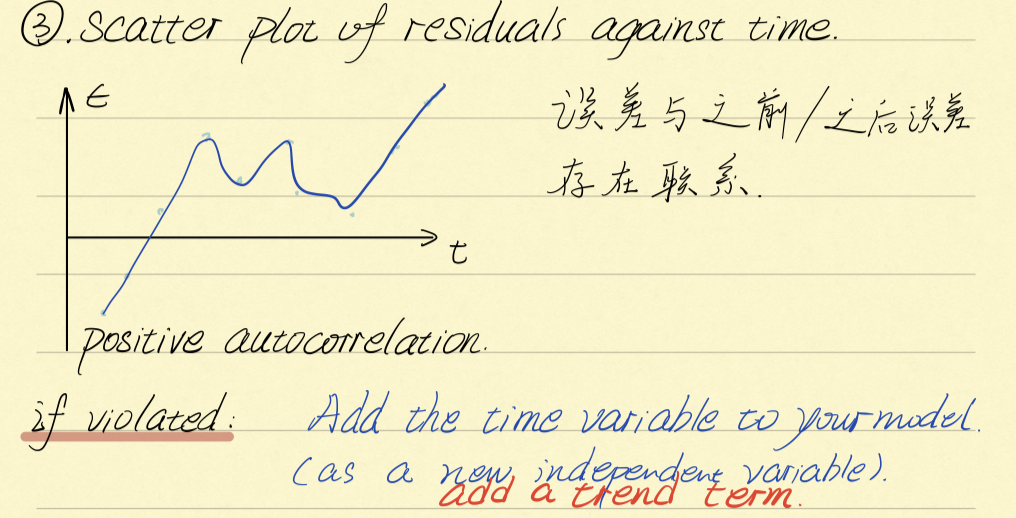
\includegraphics[scale=0.7]{check3.png}
    \caption{}
    \label{}
\end{figure}\end{center}
If violates No-Autocorrelation: add a new independent vaiable ($t$).
\subsubsection{Method 2: Durbin Watson test}
\textbf{SLR:}\\
$$d=\frac{\sum_{i=2}^n(e_i-e_{i-1})^2}{\sum_{i=1}^ne_i^2}$$
Compare $d$ with $d_L$ and $d_U$.
\begin{center}\begin{figure}[htbp]
    \centering
    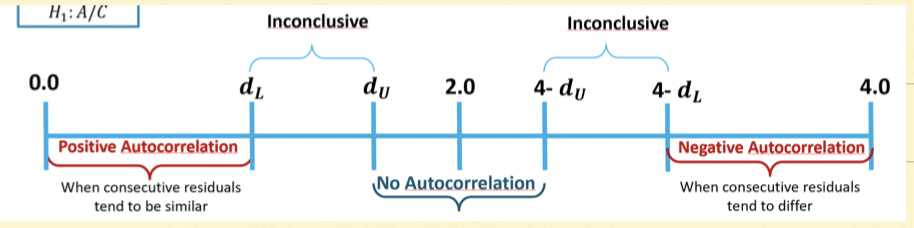
\includegraphics[scale=0.5]{check4.png}
    \caption{}
    \label{}
\end{figure}\end{center}

\textbf{MLR:}\\
$$DW=\frac{\sum_{k=1}^{n-1}(r_k-r_{k+1})^2}{\sum_{k=1}^nr_k^2}$$
if $DW<2$, then there is evidence for positive serial dependence.

\subsection{Checking Non-Linearity}
\subsubsection{Method 1: Partial Regression Plots}
We want to know \textbf{the relationship between the response $Y$ and a predictor $X_{k}$} after the effect of the other predictors has been removed.\\
To remove the effect of the other predictors, run the following two regression models:
\begin{equation}
    \begin{aligned}
        Y &\sim X_{1}+\ldots+X_{i-1}+X_{i+1}+\ldots &(1)\\
X_{i} &\sim X_{1}+\ldots+X_{i-1}+X_{i+1}+\ldots &(2)
    \end{aligned}
    \nonumber
\end{equation}

Get the following residuals:
$$
\begin{aligned}
\mathbf{r}_{y} &=\text { residuals from }(1) \\
\mathbf{r}_{k}^{X} &=\text { residuals from }(2)
\end{aligned}
$$
Plot $\mathbf{r}_{y}$ vs. $\mathbf{r}_{k}^{X}$ : For a valid model, the added-variable plot should produce points randomly scattered around a line through the origin with slope $\hat{\beta}_{k}$. This is also a useful plot to detect \textit{high influential} data points.

\subsubsection{Remedial measure: Linearizing Transformations}
1. $\log(Y)$ vs. $\log(X)$, suitable when $\mathbb{E}(Y)=\alpha X_1^{\beta_1}...X_p^{\beta_p}$\\
2. $\log(Y)$ vs. $X$, suitable when $\mathbb{E}(Y)=\alpha \exp{\sum_j X_j\beta_j}$\\
3. $\frac{1}{Y}$ vs. $X$, suitable when $\mathbb{E}(Y)=\frac{1}{\alpha+{\sum_j X_j\beta_j}}$

\subsubsection{Remedial measure: Box-Cox Transformations of $Y$ also works}

\section{Diagnostics: Collinearity}
\subsection{Exact Collinearity/ linearly dependent}
There exists a set of constants $c_1,c_2,...,c_p$ (at least one of them is non-zero) s.t.
$$\sum_{j=1}^pc_j \mathbf{X}_{.j}=0$$
then the columns of X are called \textit{linearly dependent} and there is \textit{exact collinearity}.

\subsection{What happens if collinearity}
1. $(\mathbf{X}^T \mathbf{X})^{-1}$ does not exists.\\
2. The LS estimate $\hat{beta}$ is not unique.\\
3. The corresponding linear model is not identifiable.

\subsection{Approximate Collinearity}
We generally do not need to worry about exact collinearity ($\mathbf{R}$ can detect it and fix it automatically), but \textit{approximate collinearity}.
$$\sum_{j=1}^pc_j \mathbf{X}_{.j}\approx 0$$
$$\mathbf{X}_{.k}\approx -\sum_{j\neq k}c_j \mathbf{X}_{.j}/c_k$$
A simple diagnostic for this is to obtain the regression of $\mathbf{X}_{.k}$ on the remaining predictors, and if the corresponding $R_k^2$ is close to $1$, we would diagnose approximate collinearity.
$$\mathbf{X}_{.k}\sim X_{1}+\ldots+X_{i-1}+X_{i+1}+\ldots$$




































































































































































































\end{document}